%  article.tex (Version 3.3, released 19 January 2008)
%  Article to demonstrate format for SPIE Proceedings
%  Special instructions are included in this file after the
%  symbol %>>>>
%  Numerous commands are added out, but included to show how
%  to effect various options, e.g., to print page numbers, etc.
%  This LaTeX source file is composed for LaTeX2e.

%  The following commands have been added in the SPIE class
%  file (spie.cls) and will not be understood in other classes:
%  \supit{}, \authorinfo{}, \skiplinehalf, \keywords{}
%  The bibliography style file is called spiebib.bst,
%  which replaces the standard style unstr.bst.

%\documentclass[a4paper]{spie}
\documentclass[]{spie}  %>>> use for US letter paper
%%\documentclass[a4paper]{spie}  %>>> use this instead for A4 paper
%%\documentclass[nocompress]{spie}  %>>> to avoid compression of citations
%% \addtolength{\voffset}{9mm}   %>>> moves text field down
%% \renewcommand{\baselinestretch}{1.65}   %>>> 1.65 for double spacing, 1.25 for 1.5 spacing
%  The following command loads a graphics package to include images
%  in the document. It may be necessary to specify a DVI driver option,
%  e.g., [dvips], but that may be inappropriate for some LaTeX
%  installations.
\usepackage[]{graphicx}
\usepackage{color}
\usepackage{cancel}
\usepackage{amsmath}
\usepackage{amsfonts}
\usepackage{mathtools}
\usepackage{verbatim}
\usepackage{titlesec}
\definecolor{linkcolor}{cmyk}{1, 0.65, 0, 0.3}			% PANTONE 288 CVU
\definecolor{citecolor}{cmyk}{0.79, 0, 0.87, 0.56}		% PANTONE 357 CVU
%\definecolor{citecolor}{cmyk}{1, 0, 0.47, 0.3}			% PANTONE 328
\def\red{\textcolor{red}}
\def\blue{\textcolor{blue}}
\usepackage[
	colorlinks,
	linkcolor=linkcolor,
	urlcolor=linkcolor,
	citecolor=linkcolor,
	pdftex,
	pdfstartview=FitH,
]{hyperref}

\titleformat{\section}{\normalfont\fontsize{11.5pt}{1em}\bfseries}{SUPPLEMENTARY NOTE \thesection: }{0em}{}
\titleformat{\subsection}{\normalfont\fontsize{11pt}{0.75em}\bfseries}{SUPPLEMENTARY NOTE \thesubsection: }{0em}{}
\titleformat{\subsubsection}{\normalfont\fontsize{11pt}{0.75em}\bfseries}{SUPPLEMENTARY NOTE \thesubsubsection: }{0em}{}

% jump to the top of a figure, not the caption
\usepackage[all]{hypcap}

% so that footnotes in tables work
\usepackage{footnote}

% so that we can omit the 'Table 1:' for the overview
\usepackage{caption}

% should be called Supplementary Figure
\renewcommand{\figurename}{Supplementary Figure}

% for the source code
\usepackage{listings}

\usepackage{helvet}
\renewcommand{\rmdefault}{\sfdefault}
\renewcommand{\baselinestretch}{1.05}

%\usepackage{sectsty}Bayesian-based single-view and multi-view deconvolution
%\allsectionsfont{\sffamily}

\captionsetup[table]{labelformat=empty}

\newcommand\smallurl[1]{{\small{\url{#1}}}}
\newcommand\tablespace{\vspace{2.5mm}}
\newcommand\fig{supplementary figure }
\newcommand\Fig{Supplementary figure }


\title{BigStitcher: Efficient alignment of large multi-tile and multi-view image datasets}

%>>>> The author is responsible for formatting the
%  author list and their institutions.  Use  \skiplinehalf
%  to separate author list from addresses and between each address.
%  The correspondence between each author and his/her address
%  can be indicated with a superscript in italics,
%  which is easily obtained with \supit{}.

\author{David H{\"o}rl, Fabio Rojas Rusak, Stephan Preibisch
%\skiplinehalf
%\small{
%\supit{1}Max Planck Institute of Molecular Cell Biology and Genetics, Pfotenhauerstrasse 108, Dresden, Germany \\
%\supit{2}HHMI Janelia Farm Research Campus, 19700 Helix Drive, Ashburn, VA 20147, USA \\
%\supit{3}Albert Einstein College of Medicine, 1300 Morris Park Avenue, Bronx, NY 10461, USA
%}
}

%>>>> Further information about the authors, other than their
%  institution and addresses, should be included as a footnote,
%  which is facilitated by the \authorinfo{} command.

%\authorinfo{Further author information: (Send correspondence to A.A.A.)\\A.A.A.: E-mail: aaa@tbk2.edu, Telephone: 1 505 123 1234\\  B.B.A.: E-mail: bba@cmp.com, Telephone: +33 (0)1 98 76 54 32}
%%>>>> when using amstex, you need to use @@ instead of @


%%%%%%%%%%%%%%%%%%%%%%%%%%%%%%%%%%%%%%%%%%%%%%%%%%%%%%%%%%%%%
%>>>> uncomment following for page numbers
\pagestyle{plain}
%>>>> uncomment following to start page numbering at 301
%\setcounter{page}{1}

% underset argument for (arg)max/min
\DeclareMathOperator*{\argmax}{arg\,max}
\DeclareMathOperator*{\argmin}{arg\,min}
%\DeclareMathOperator*{\max}{max}
%\DeclareMathOperator*{\min}{min}
%\DeclareMathOperator{\deg}{deg}






\begin{document}

\maketitle

%\pagestyle{headings}
\setcounter{page}{1}
\pagenumbering{roman}
\pagenumbering{arabic}


\hspace{20mm}

\begin{table}[h!]
\center
{
\fontsize{12pt}{11pt}\selectfont
\center
\begin{tabular}{lp{11cm}}
\textbf{\textcolor{red}{Supplementary File}} & \textbf{\textcolor{red}{Title}}\\ \\
\hline
\\
\textbf{Supplementary Figure \ref{fig:sup-fig-rf}} & Fluorescence in cleared sample? Random Forest? \tablespace \\
\textbf{Supplementary Figure \ref{fig:sup-fig-illu-select}} & Illumination selection \tablespace \\
\textbf{Supplementary Figure \ref{fig:sup-fig-manual-align1}} &  Manual alignment \tablespace \\
\textbf{Supplementary Figure \ref{fig:sup-fig-flatfield}} & Flat-field correction \tablespace \\
\textbf{Supplementary Figure \ref{fig:sup-fig-stitching}} & Pairwise registration by phase correlation \tablespace \\
\textbf{Supplementary Figure \ref{fig:sup-fig-downsampling}} & Downsampling with different SNR \tablespace \\
\textbf{Supplementary Figure \ref{fig:sup-fig-downsampling-statistics-1}} & Downsampling error statistics 1 \tablespace \\
\textbf{Supplementary Figure \ref{fig:sup-fig-downsampling-statistics-2}} & Downsampling error statistics 2 \tablespace \\
\textbf{Supplementary Figure \ref{fig:sup-fig-link-explorer}} & Interactive inspection and curation of pairwise links \tablespace \\
\textbf{Supplementary Figure \ref{fig:sup-fig-globalopt}} & Global optimization \tablespace \\
\textbf{Supplementary Figure \ref{fig:sup-fig-icp}} & Affine refinement via ICP \tablespace \\
\textbf{Supplementary Figure \ref{fig:sup-fig-interest-point}} & Interest point visualization \tablespace \\
\textbf{Supplementary Figure \ref{fig:sup-fig-manual-align2}} & Manual Transformation of multi-view datasets \tablespace \\
\textbf{Supplementary Figure \ref{fig:sup-fig-boundingbox}} & Bounding Box definition \tablespace \\
\textbf{Supplementary Figure \ref{fig:sup-fig-fusion}} & Virtual fusion of large image \tablespace \\
\textbf{Supplementary Note \ref{sec:sup-methods}} & Supplementary methods \tablespace \\
\textbf{Supplementary Note \ref{sec:documentation}} & BigStitcher User Guide \tablespace \\
\textbf{Supplementary Note \ref{sec:currentcode}} & Links to the current source codes \tablespace \\

\end{tabular}}
\caption{\emph{Note: Supplementary Videos 1--XXX are available for download on the journal homepage.}}
\end{table}

\pagebreak

\titleformat{\section}{\centering\normalfont\fontsize{11.5pt}{1em}\bfseries}{SUPPLEMENTARY NOTE \thesection: }{0em}{}
\section*{SUPPLEMENTARY FIGURES}
\titleformat{\section}{\normalfont\fontsize{11.5pt}{1em}\bfseries}{SUPPLEMENTARY NOTE \thesection: }{0em}{}


\subsection*{SUPPLEMENTARY FIGURE 1: Fluorescence in cleared sample??}
\vspace{1mm}
\begin{figure*}[h!]
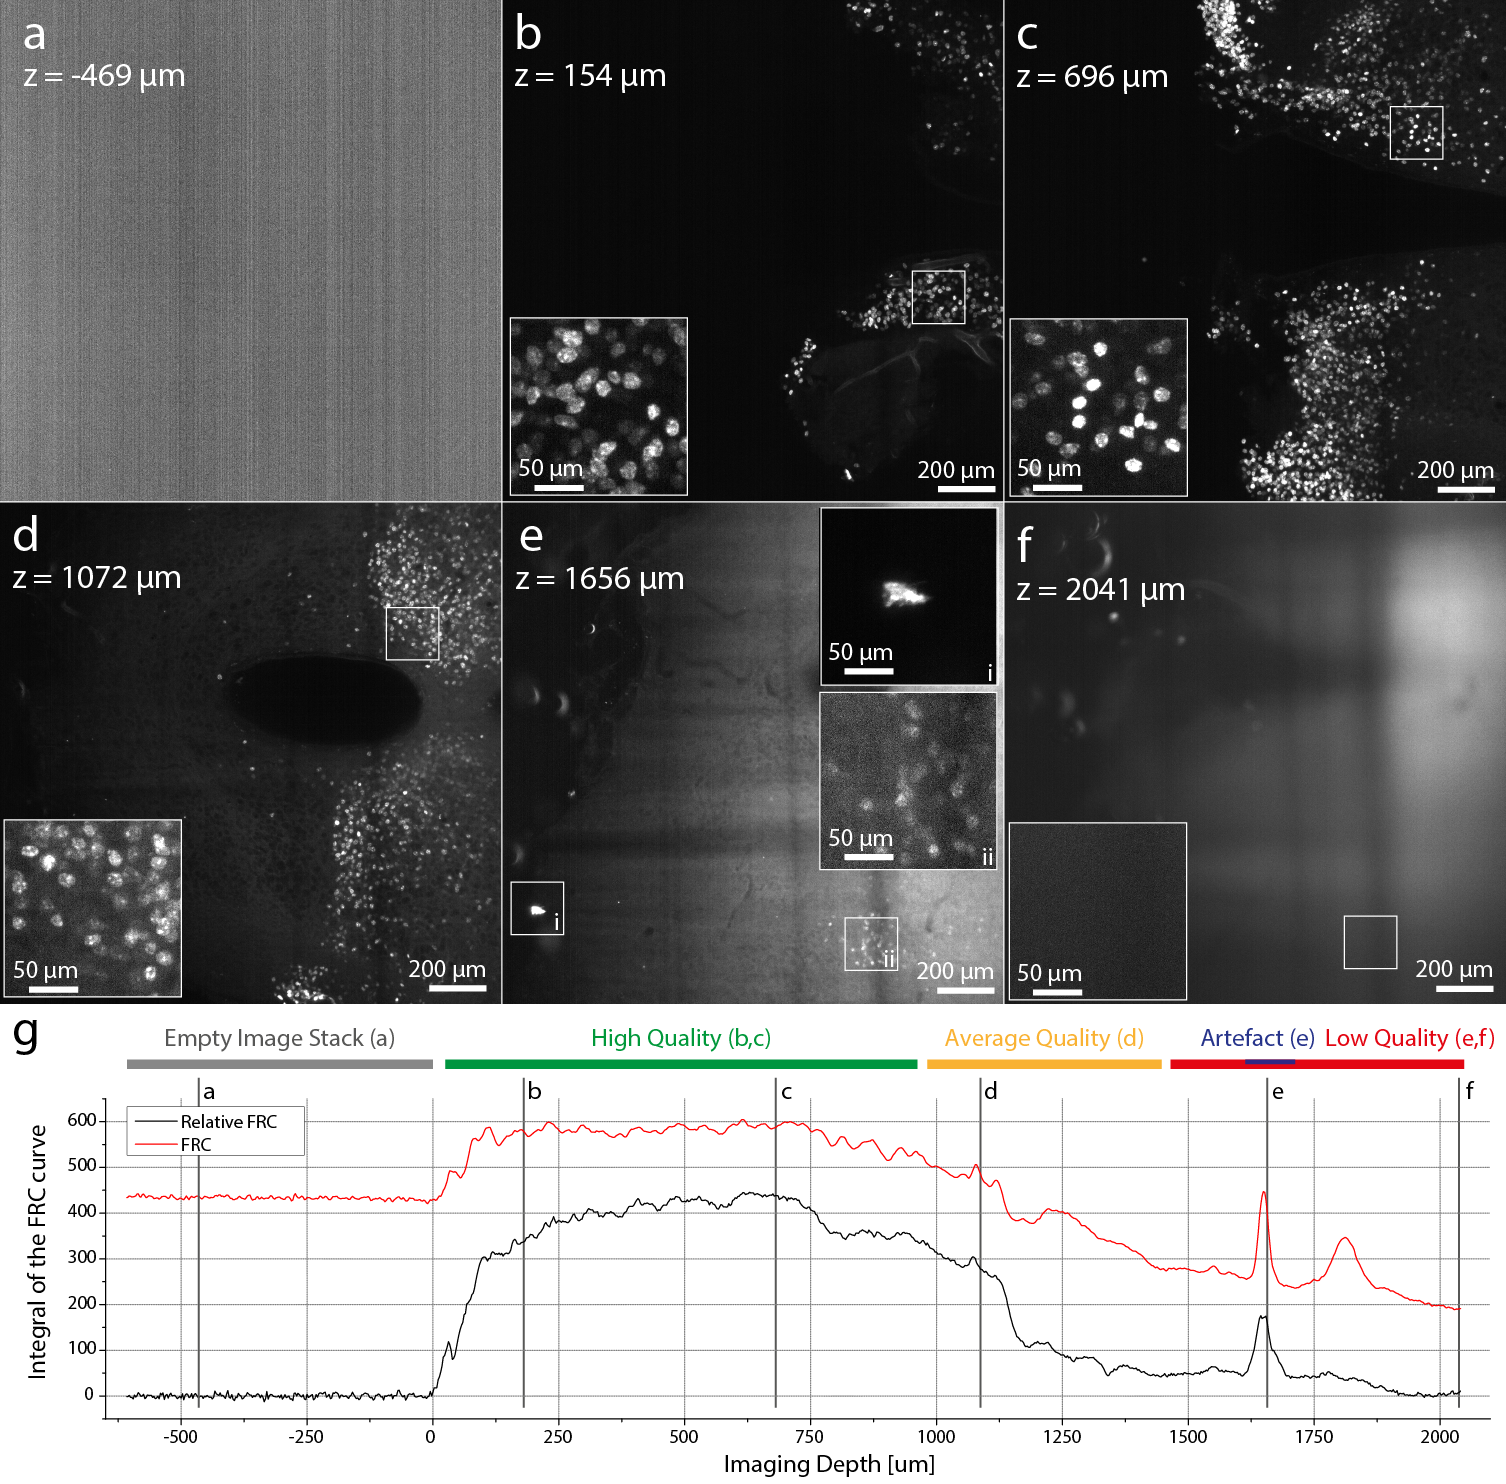
\includegraphics[width=\textwidth]{fig-rf.png}
\vspace{-2.0mm}
\caption{\hspace{-0.5mm} \emph{Lorem ipsum.} Dolor sit amet.
}
\label{fig:sup-fig-rf}
\end{figure*}

\pagebreak


\subsection*{SUPPLEMENTARY FIGURE 2: Illumination selection}
\vspace{1mm}
\begin{figure*}[h!]
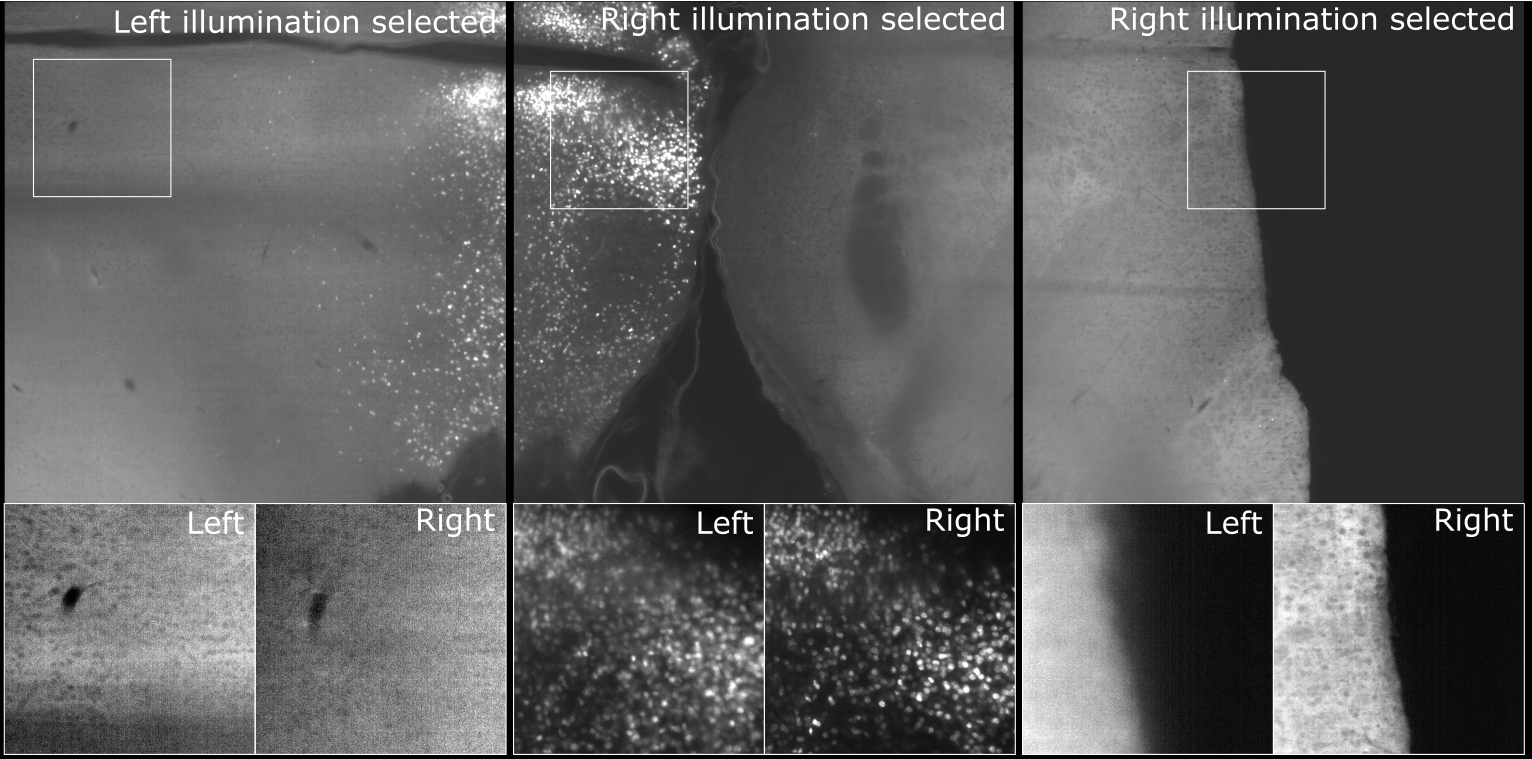
\includegraphics[width=\textwidth]{Illu_Select.png}
\vspace{-2.0mm}
\caption{\hspace{-0.5mm} \emph{Lorem ipsum.} Dolor sit amet.
}
\label{fig:sup-fig-illu-select}
\end{figure*}

\pagebreak


\subsection*{SUPPLEMENTARY FIGURE 3: Manual alignment}
\vspace{1mm}
\begin{figure*}[h!]
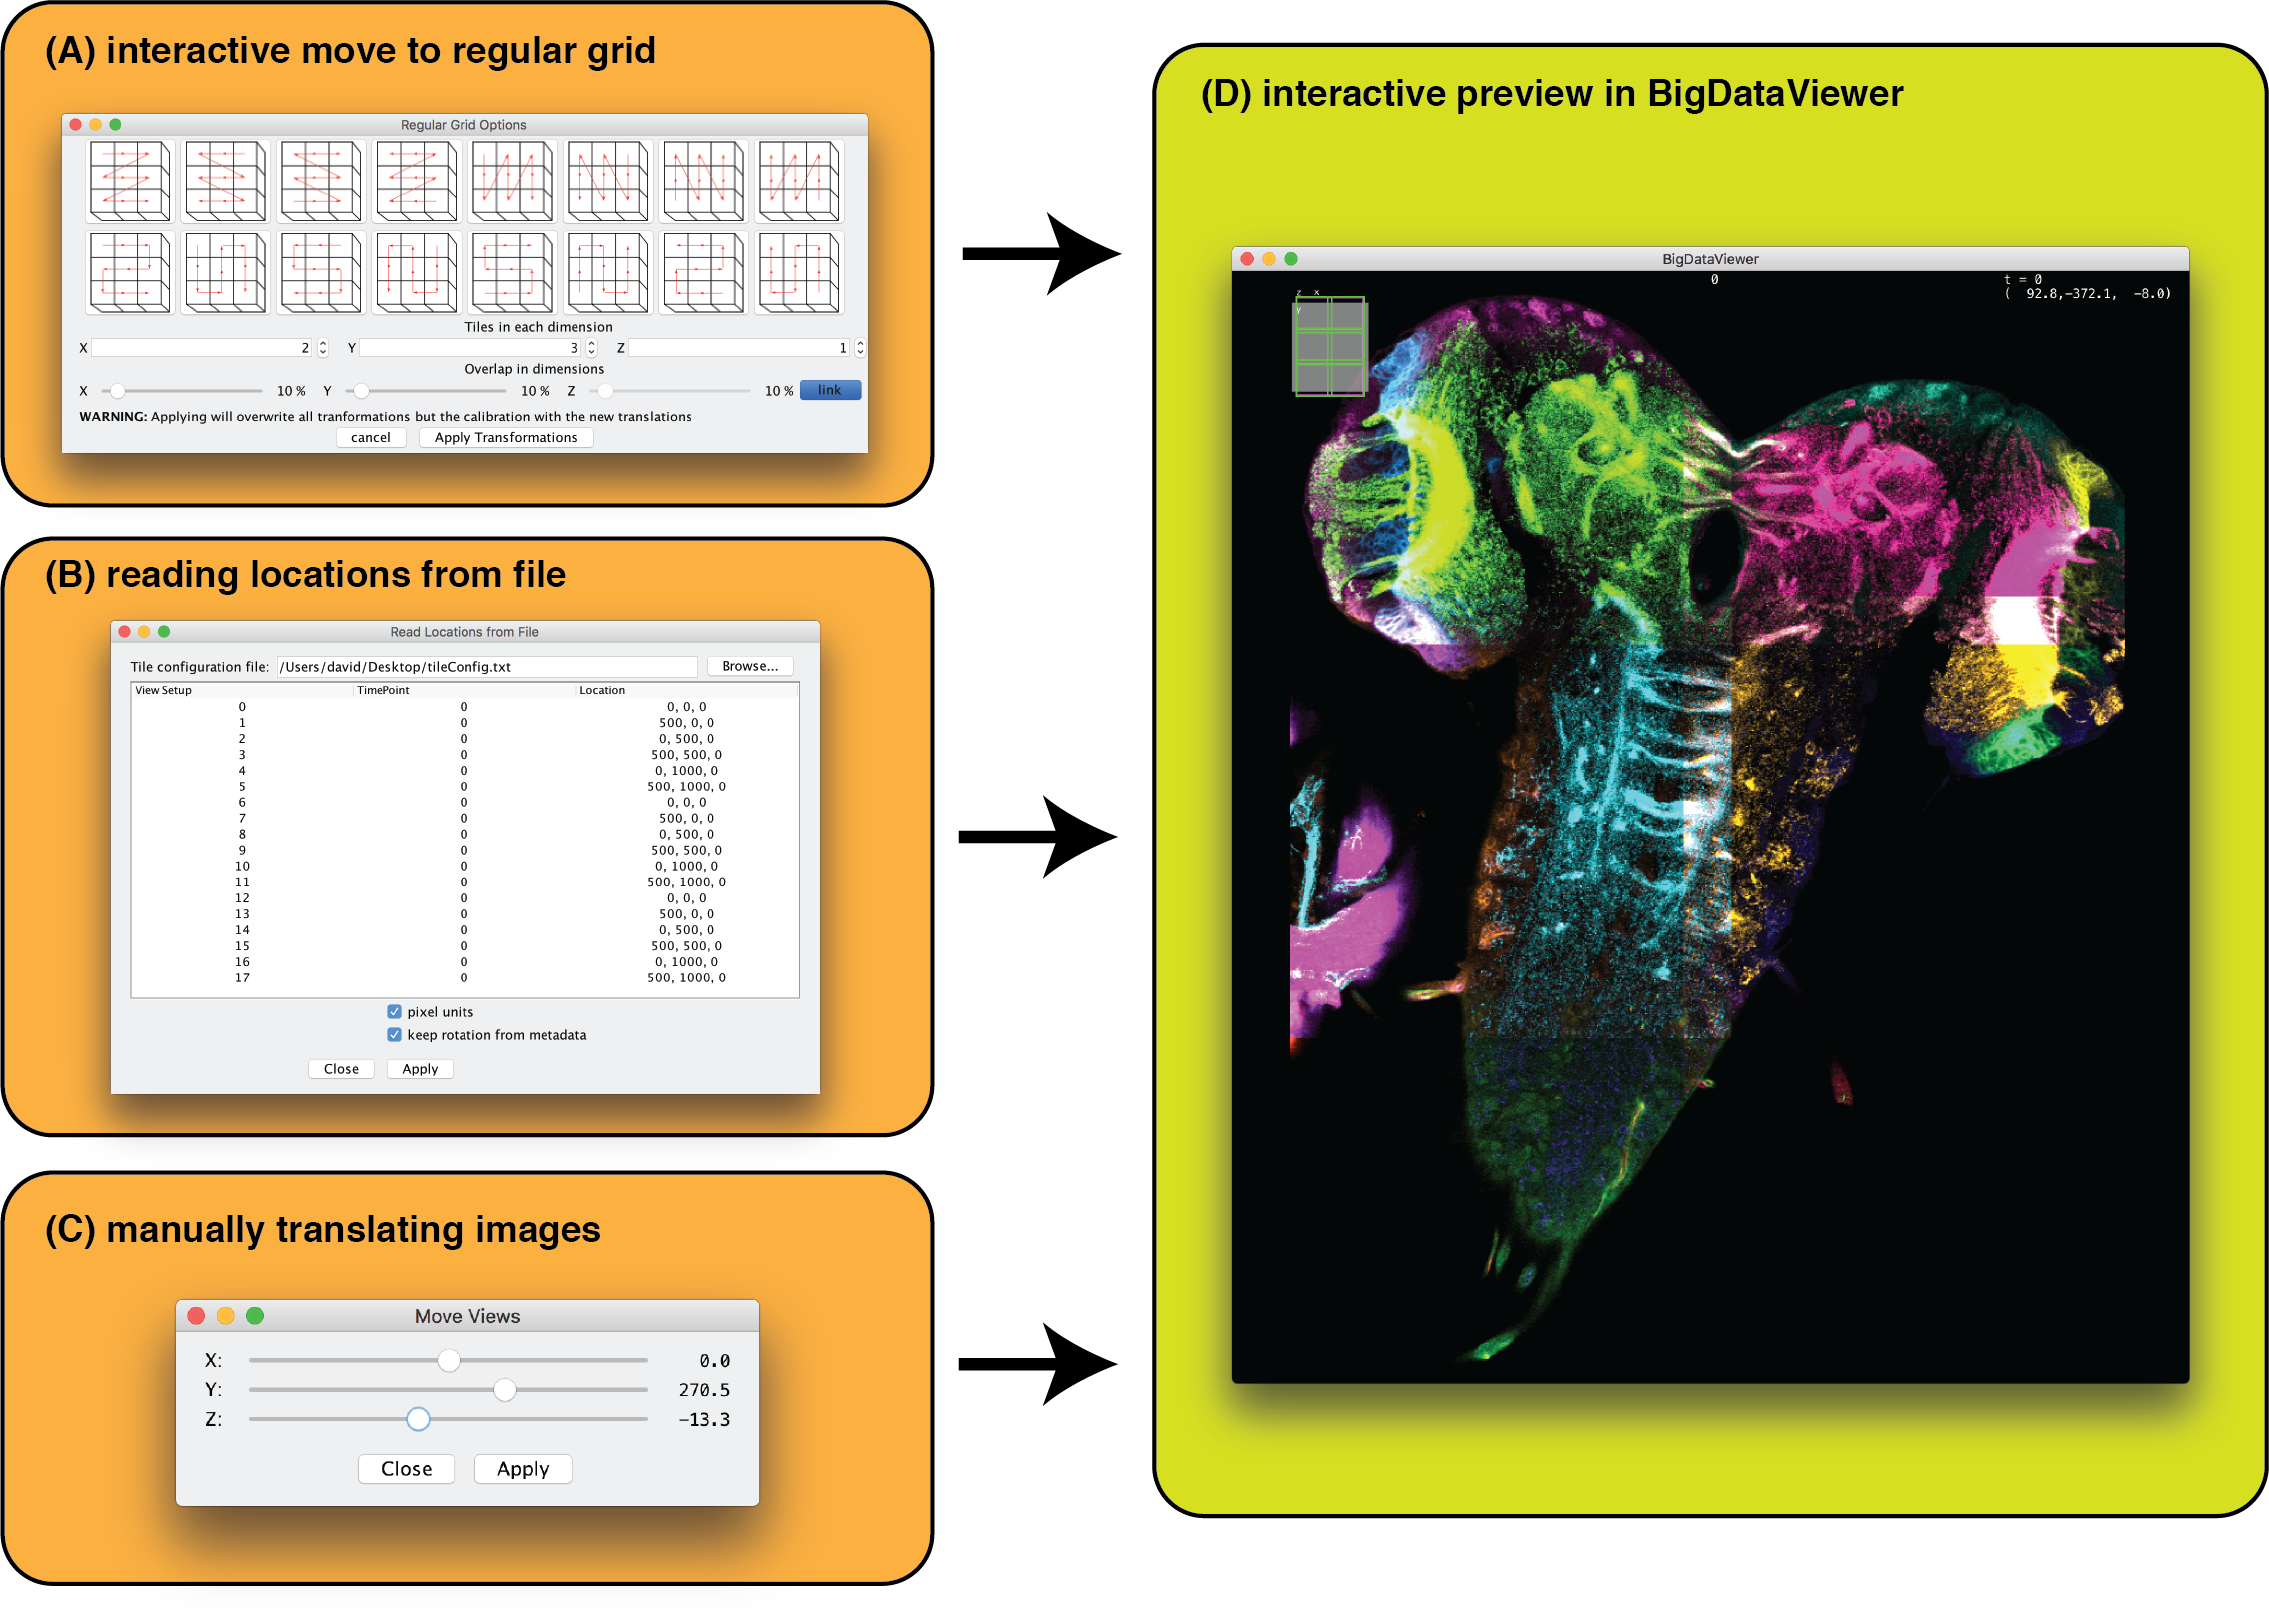
\includegraphics[width=\textwidth]{manual-view-arrangement.png}
\vspace{-2.0mm}
\caption{\hspace{-0.5mm} \emph{Interactive manual alignment of tiled images.} The BigStitcher GUI offers various ways of manually (pre-)aligning tiled images. Images can be moved to a regular grid with a given tile order and overlap \textbf{(A)}. Image locations can also be read from a simple \emph{tile configuration} text file \textbf{(B)}. Furthermore, selected image(s) can be moved along axes via sliders \textbf{(C)}. All changes will be displayed in the BigDataViewer window immediately \textbf{(D)} for quick verification. 
}
\label{fig:sup-fig-manual-align1}
\end{figure*}

\pagebreak


\subsection*{SUPPLEMENTARY FIGURE 4: Flat-field correction}
\vspace{1mm}
\begin{figure*}[h!]
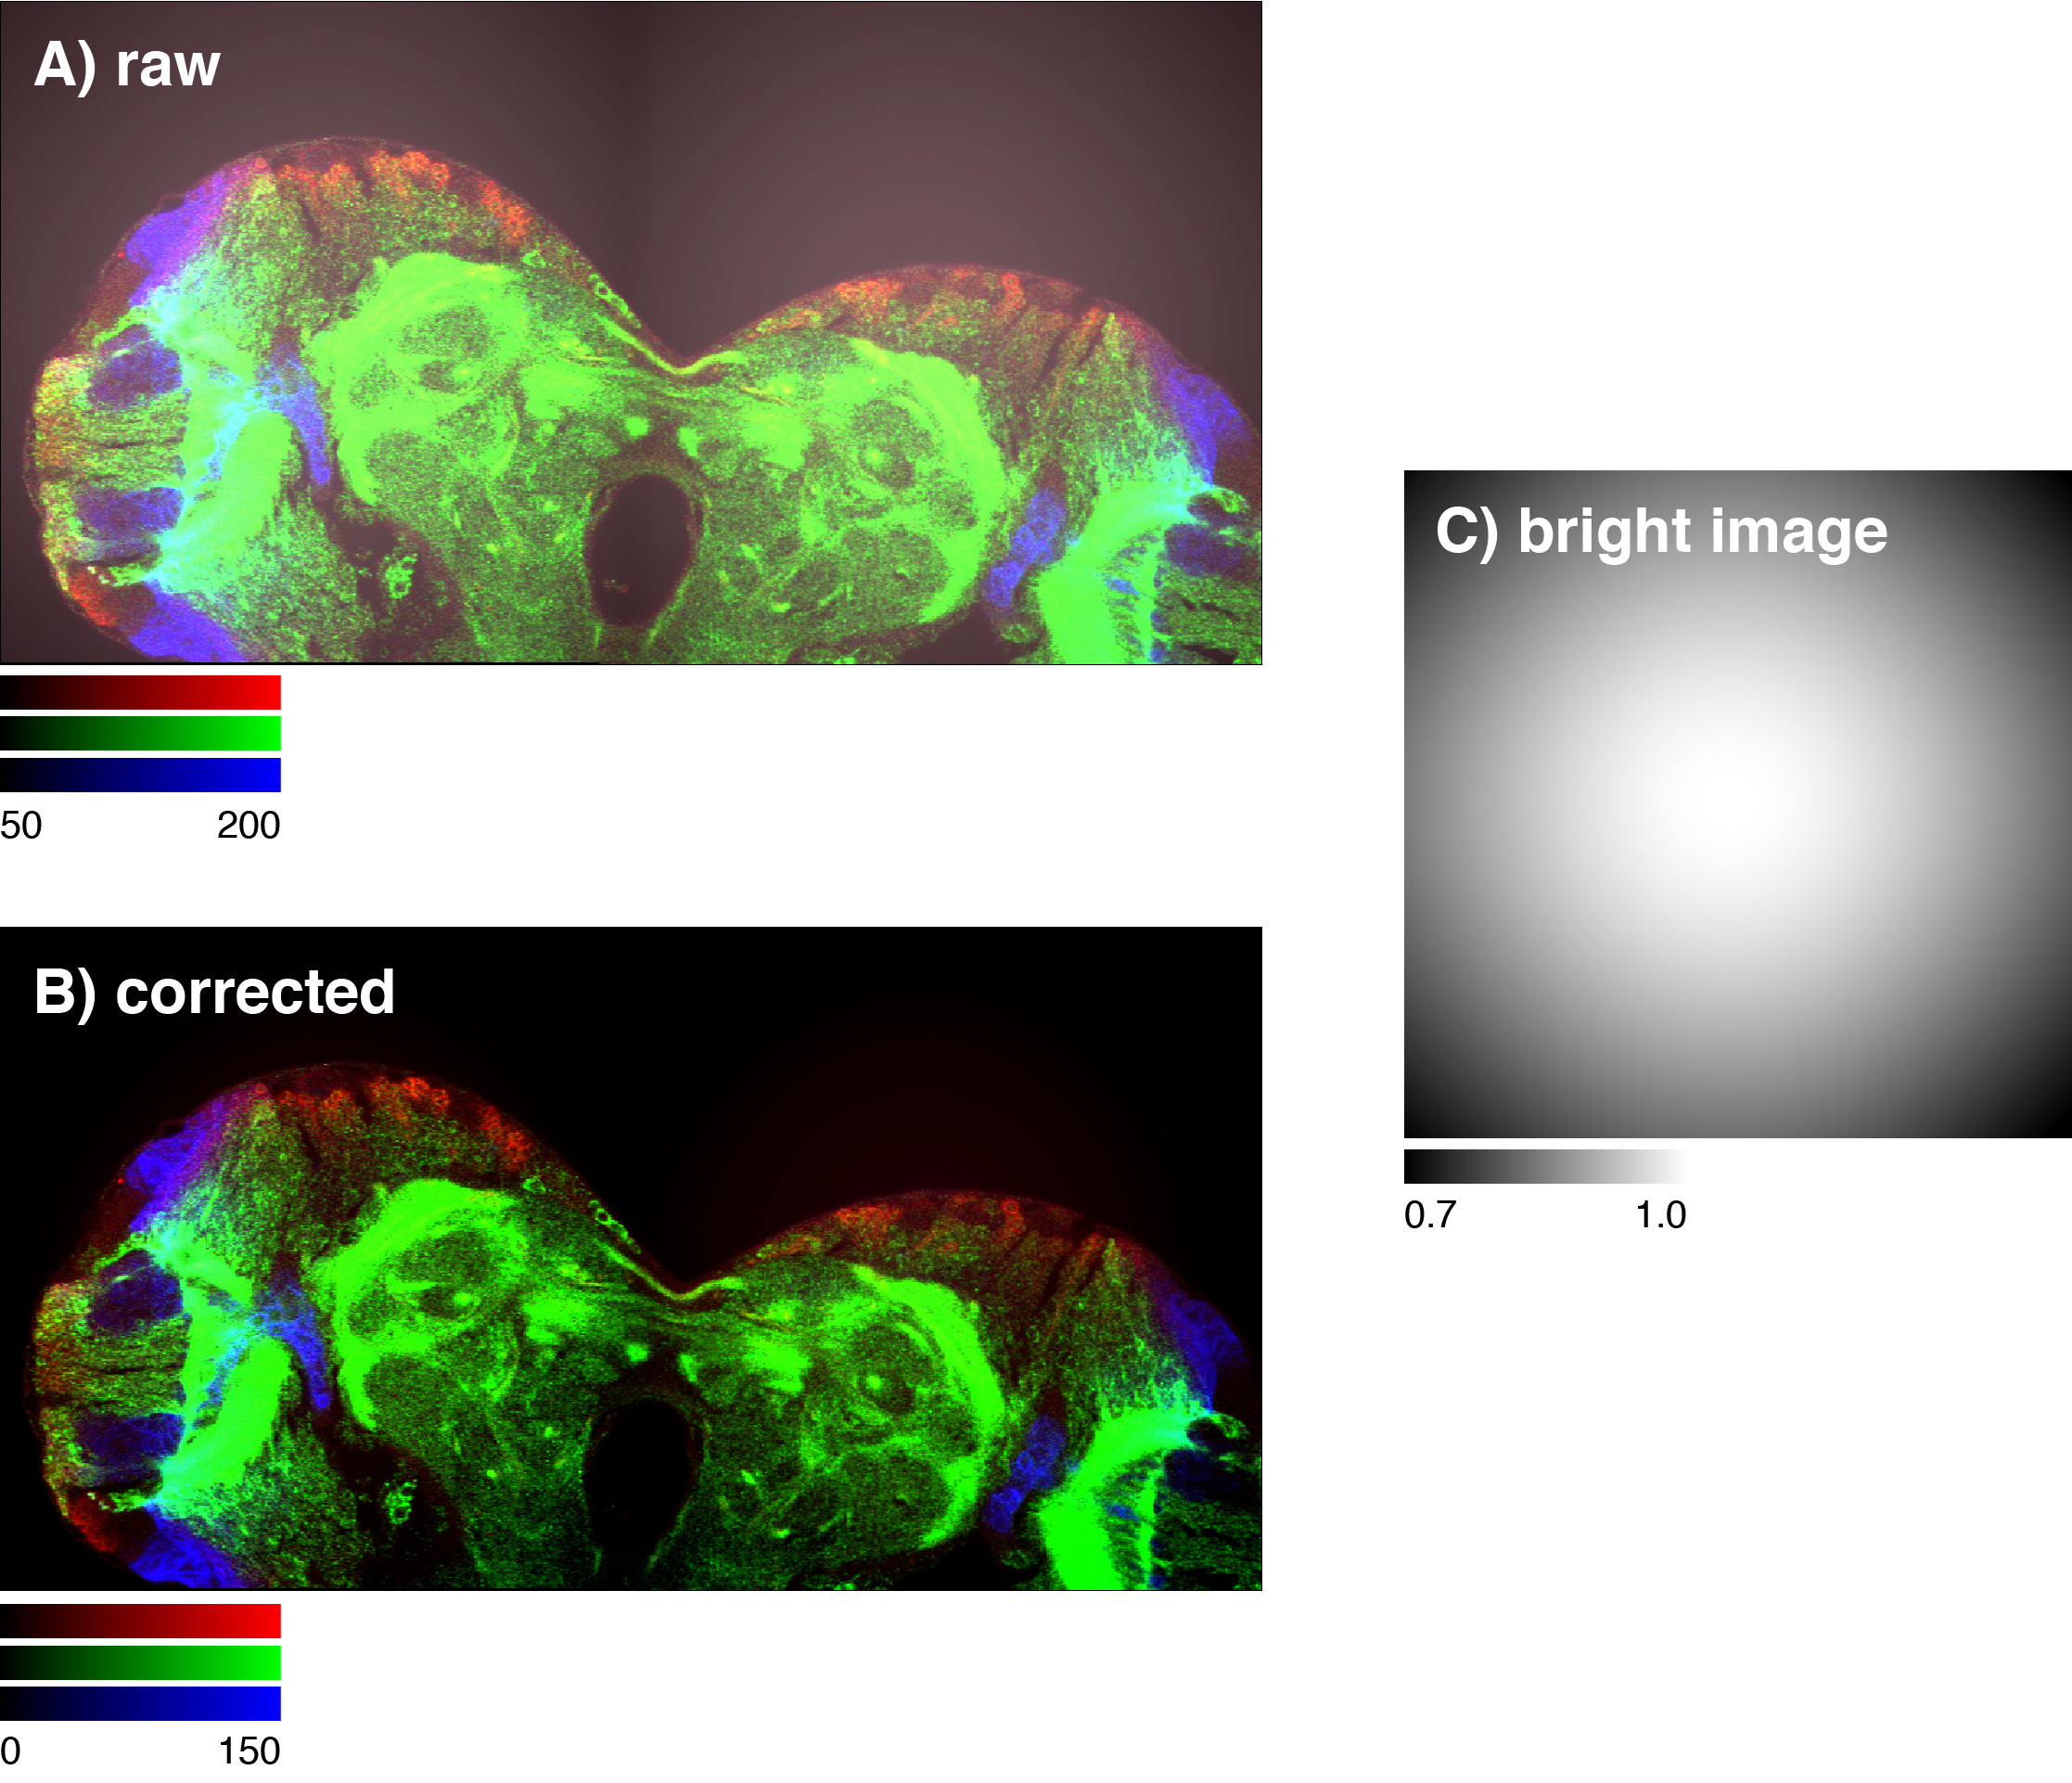
\includegraphics[width=\textwidth]{fig-flatfield.png}
\vspace{-2.0mm}
\caption{\hspace{-0.5mm} \emph{On-the-fly flat-field correction.} The BigStitcher offers correction for camera offsets, fixed pattern noise or uneven illumination. \textbf{(A):}  Simulation of the effects of a constant background offset and Gaussian illumination/detection efficiency \textbf{(C)} on tiled images. By subtracting the \emph{dark image} and modulating with the inverse relative intensity of the \emph{bright image}, such artefacts can be corrected easily \textbf{(B)}. The correction is calculated virtually, with optional cacheing, to allow for immediate inspection of the results.
}
\label{fig:sup-fig-flatfield}
\end{figure*}

\pagebreak


\subsection*{SUPPLEMENTARY FIGURE 5: Pairwise registration by phase correlation}
\vspace{1mm}
\begin{figure*}[h!]
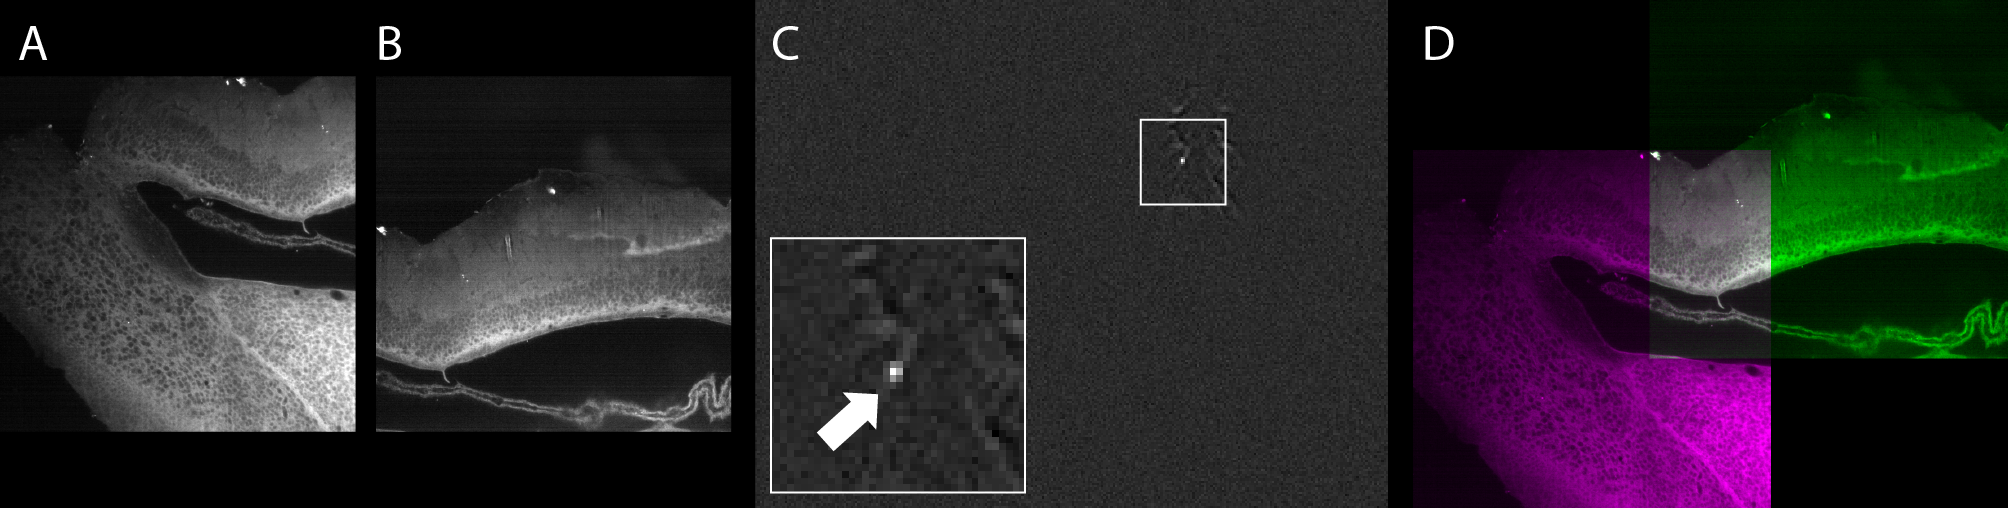
\includegraphics[width=\textwidth]{fig-stitching.png}
\vspace{-2.0mm}
\caption{\hspace{-0.5mm} \emph{Lorem ipsum.} Dolor sit amet.
}
\label{fig:sup-fig-stitching}
\end{figure*}

\pagebreak



\subsection*{SUPPLEMENTARY FIGURE 6: Downsampling with different SNR}
\vspace{1mm}
\begin{figure*}[h!]
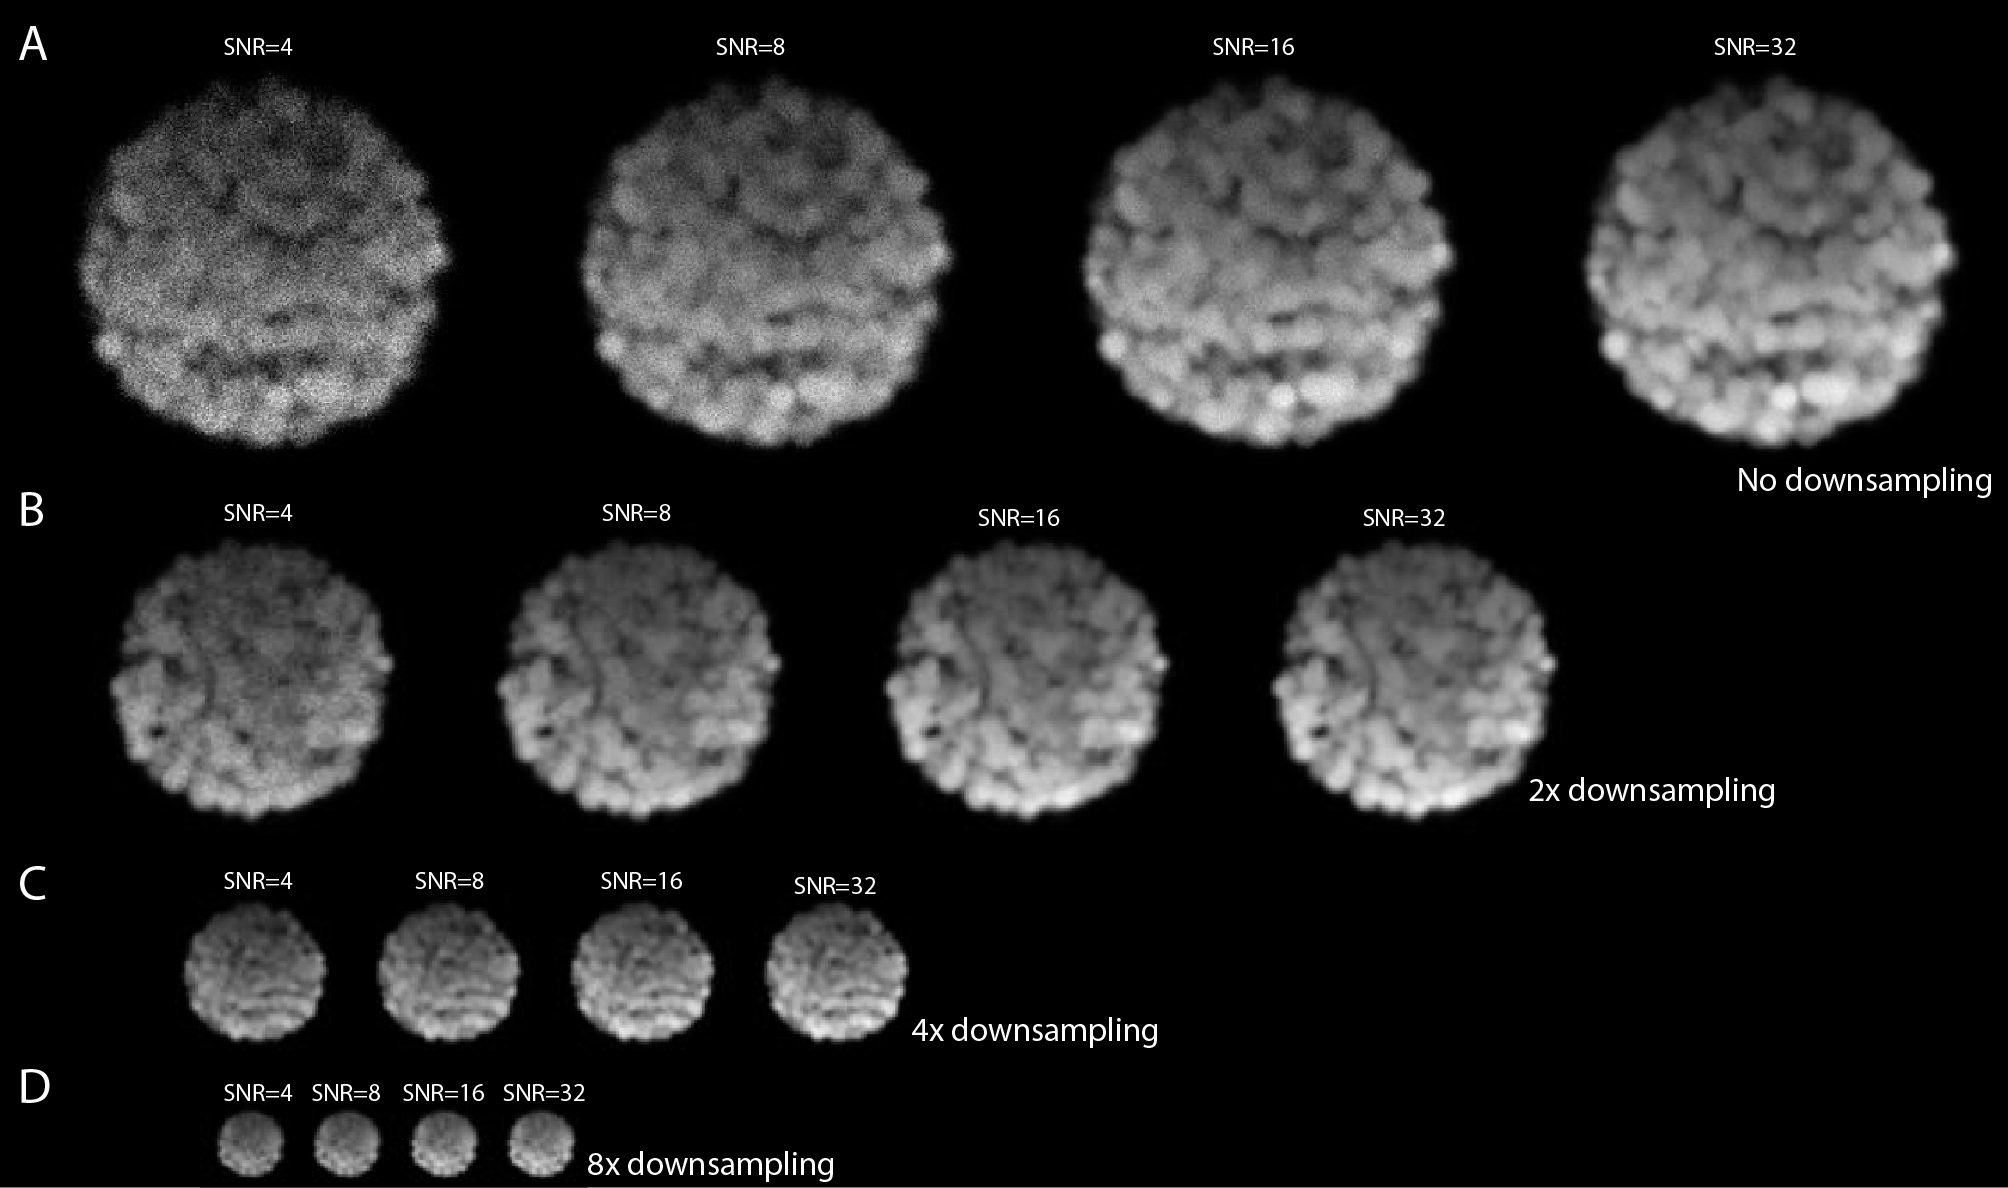
\includegraphics[width=\textwidth]{fig-downsampling.png}
\vspace{-2.0mm}
\caption{\hspace{-0.5mm} \emph{Lorem ipsum.} Dolor sit amet.
}
\label{fig:sup-fig-downsampling}
\end{figure*}

\pagebreak



\subsection*{SUPPLEMENTARY FIGURE 7: Downsampling statistics 1}
\vspace{1mm}
\begin{figure*}[h!]
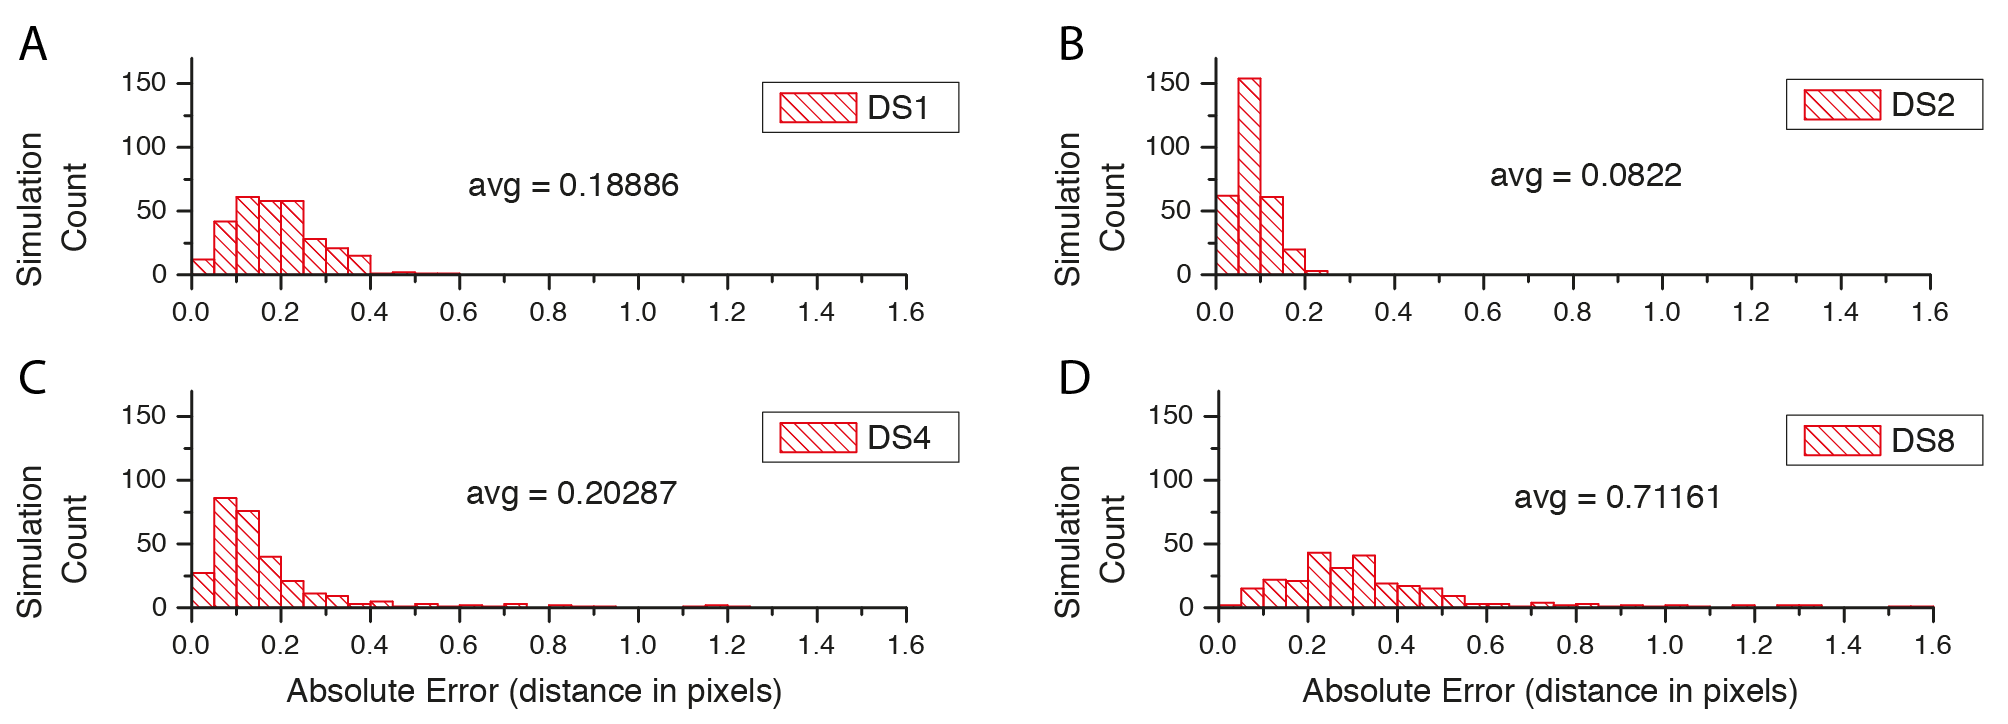
\includegraphics[width=\textwidth]{fig-downsampling-statistics-1.png}
\vspace{-2.0mm}
\caption{\hspace{-0.5mm} \emph{Lorem ipsum.} Dolor sit amet.
}
\label{fig:sup-fig-downsampling-statistics-1}
\end{figure*}

\pagebreak



\subsection*{SUPPLEMENTARY FIGURE 8: Downsampling statistics 2}
\vspace{1mm}
\begin{figure*}[h!]
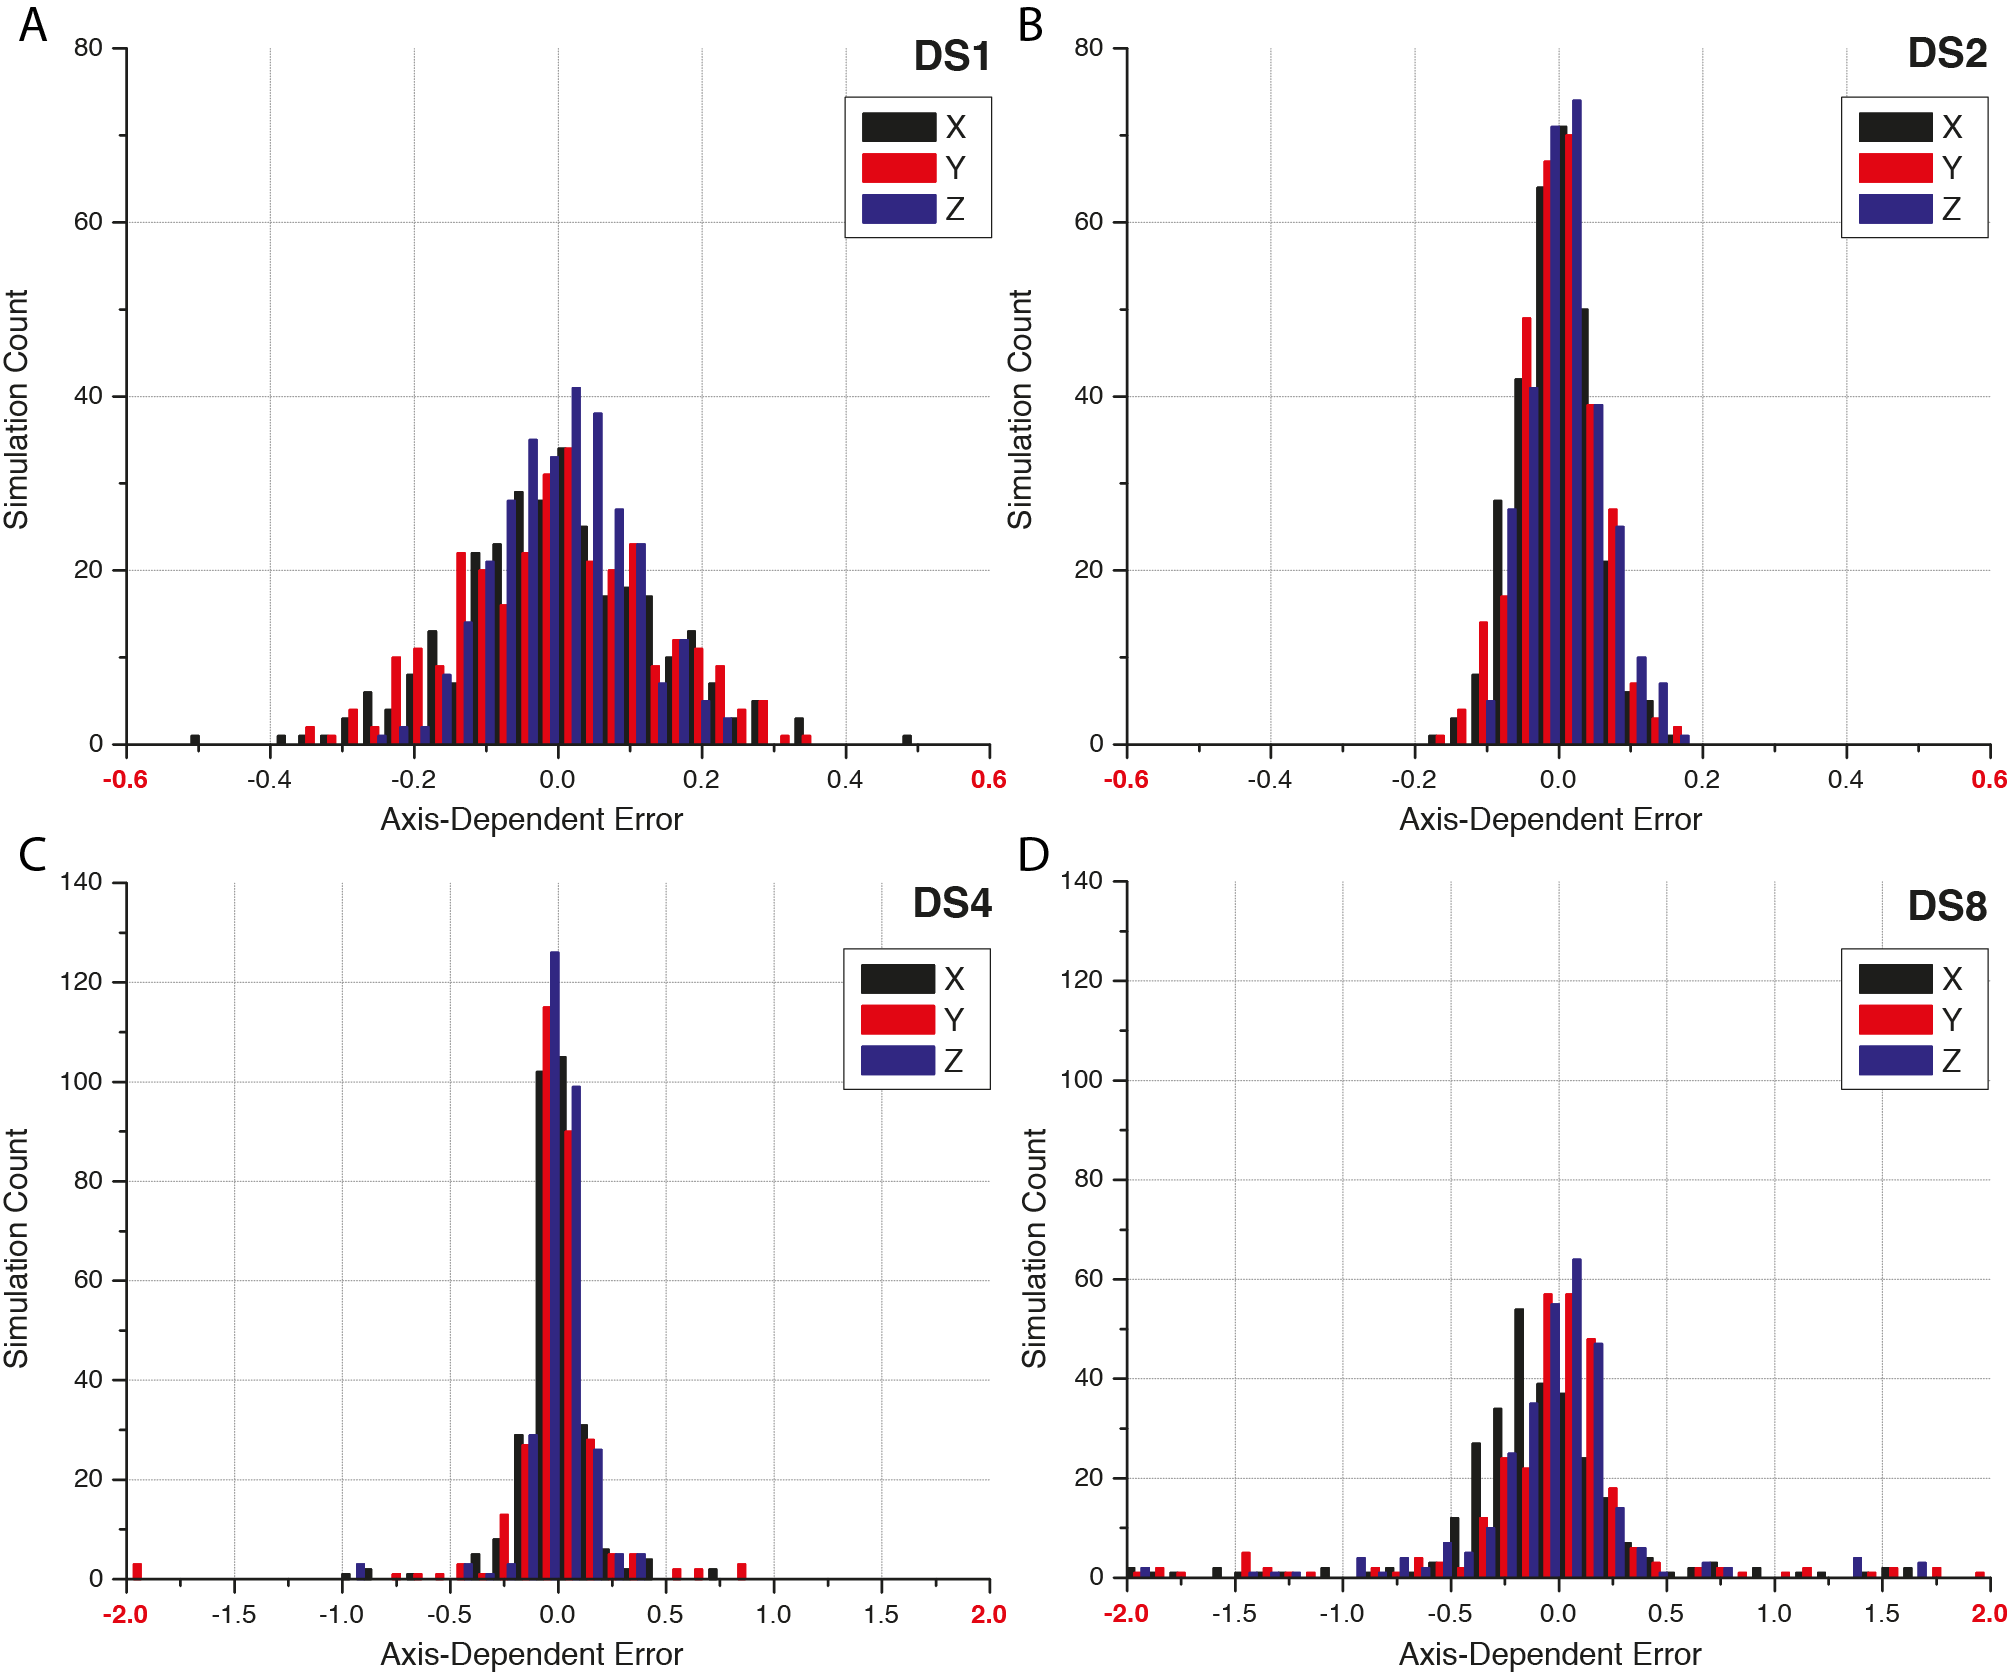
\includegraphics[width=\textwidth]{fig-downsampling-statistics-2.png}
\vspace{-2.0mm}
\caption{\hspace{-0.5mm} \emph{Lorem ipsum.} Dolor sit amet.
}
\label{fig:sup-fig-downsampling-statistics-2}
\end{figure*}

\pagebreak


\subsection*{SUPPLEMENTARY FIGURE 9: Interactive inspection and curation of pairwise links}
\vspace{1mm}
\begin{figure*}[h!]
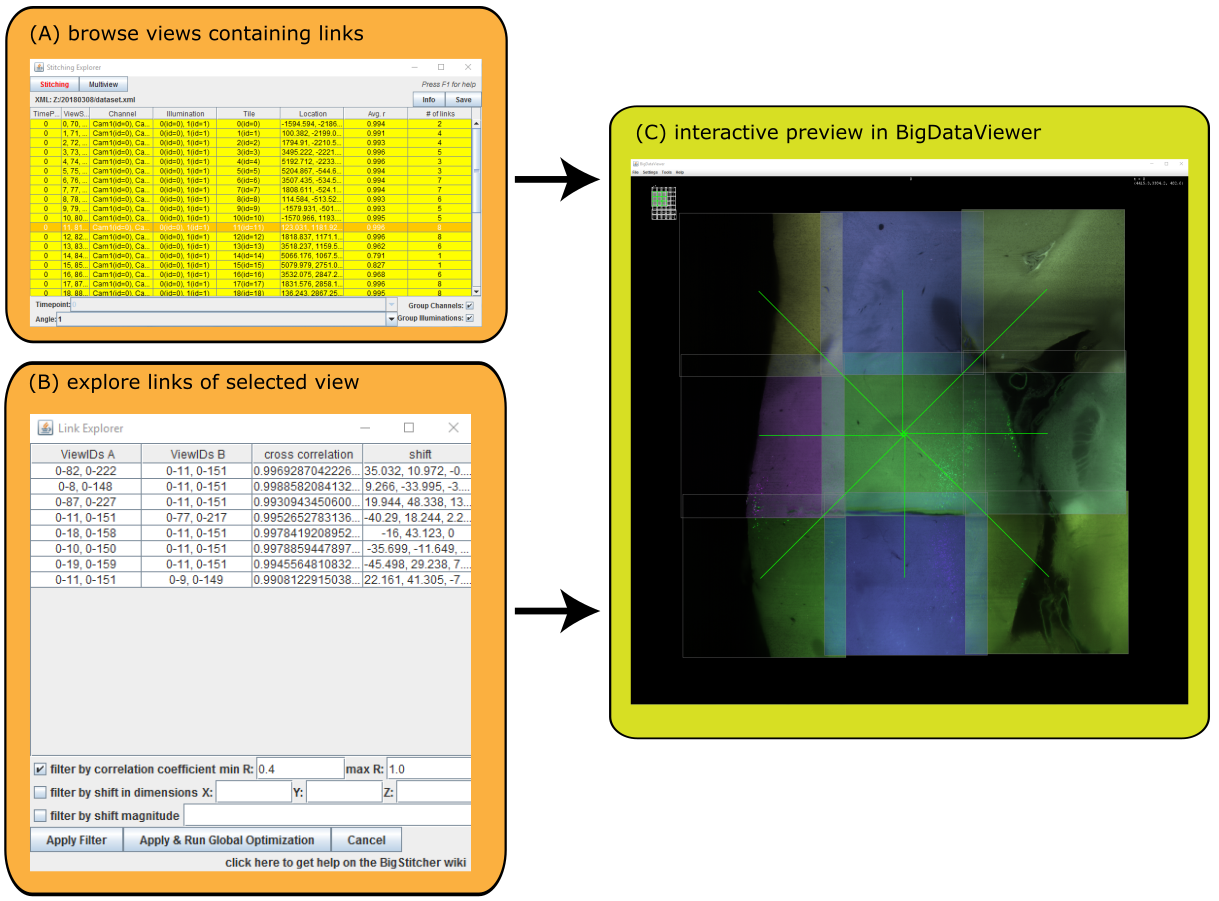
\includegraphics[width=\textwidth]{Supp-Link-Explorer.png}
\vspace{-2.0mm}
\caption{\hspace{-0.5mm} \emph{Lorem ipsum.} Dolor sit amet.
}
\label{fig:sup-fig-link-explorer}
\end{figure*}

\pagebreak


\subsection*{SUPPLEMENTARY FIGURE 10: Global optimization}
\vspace{1mm}
\begin{figure*}[h!]
\centerline{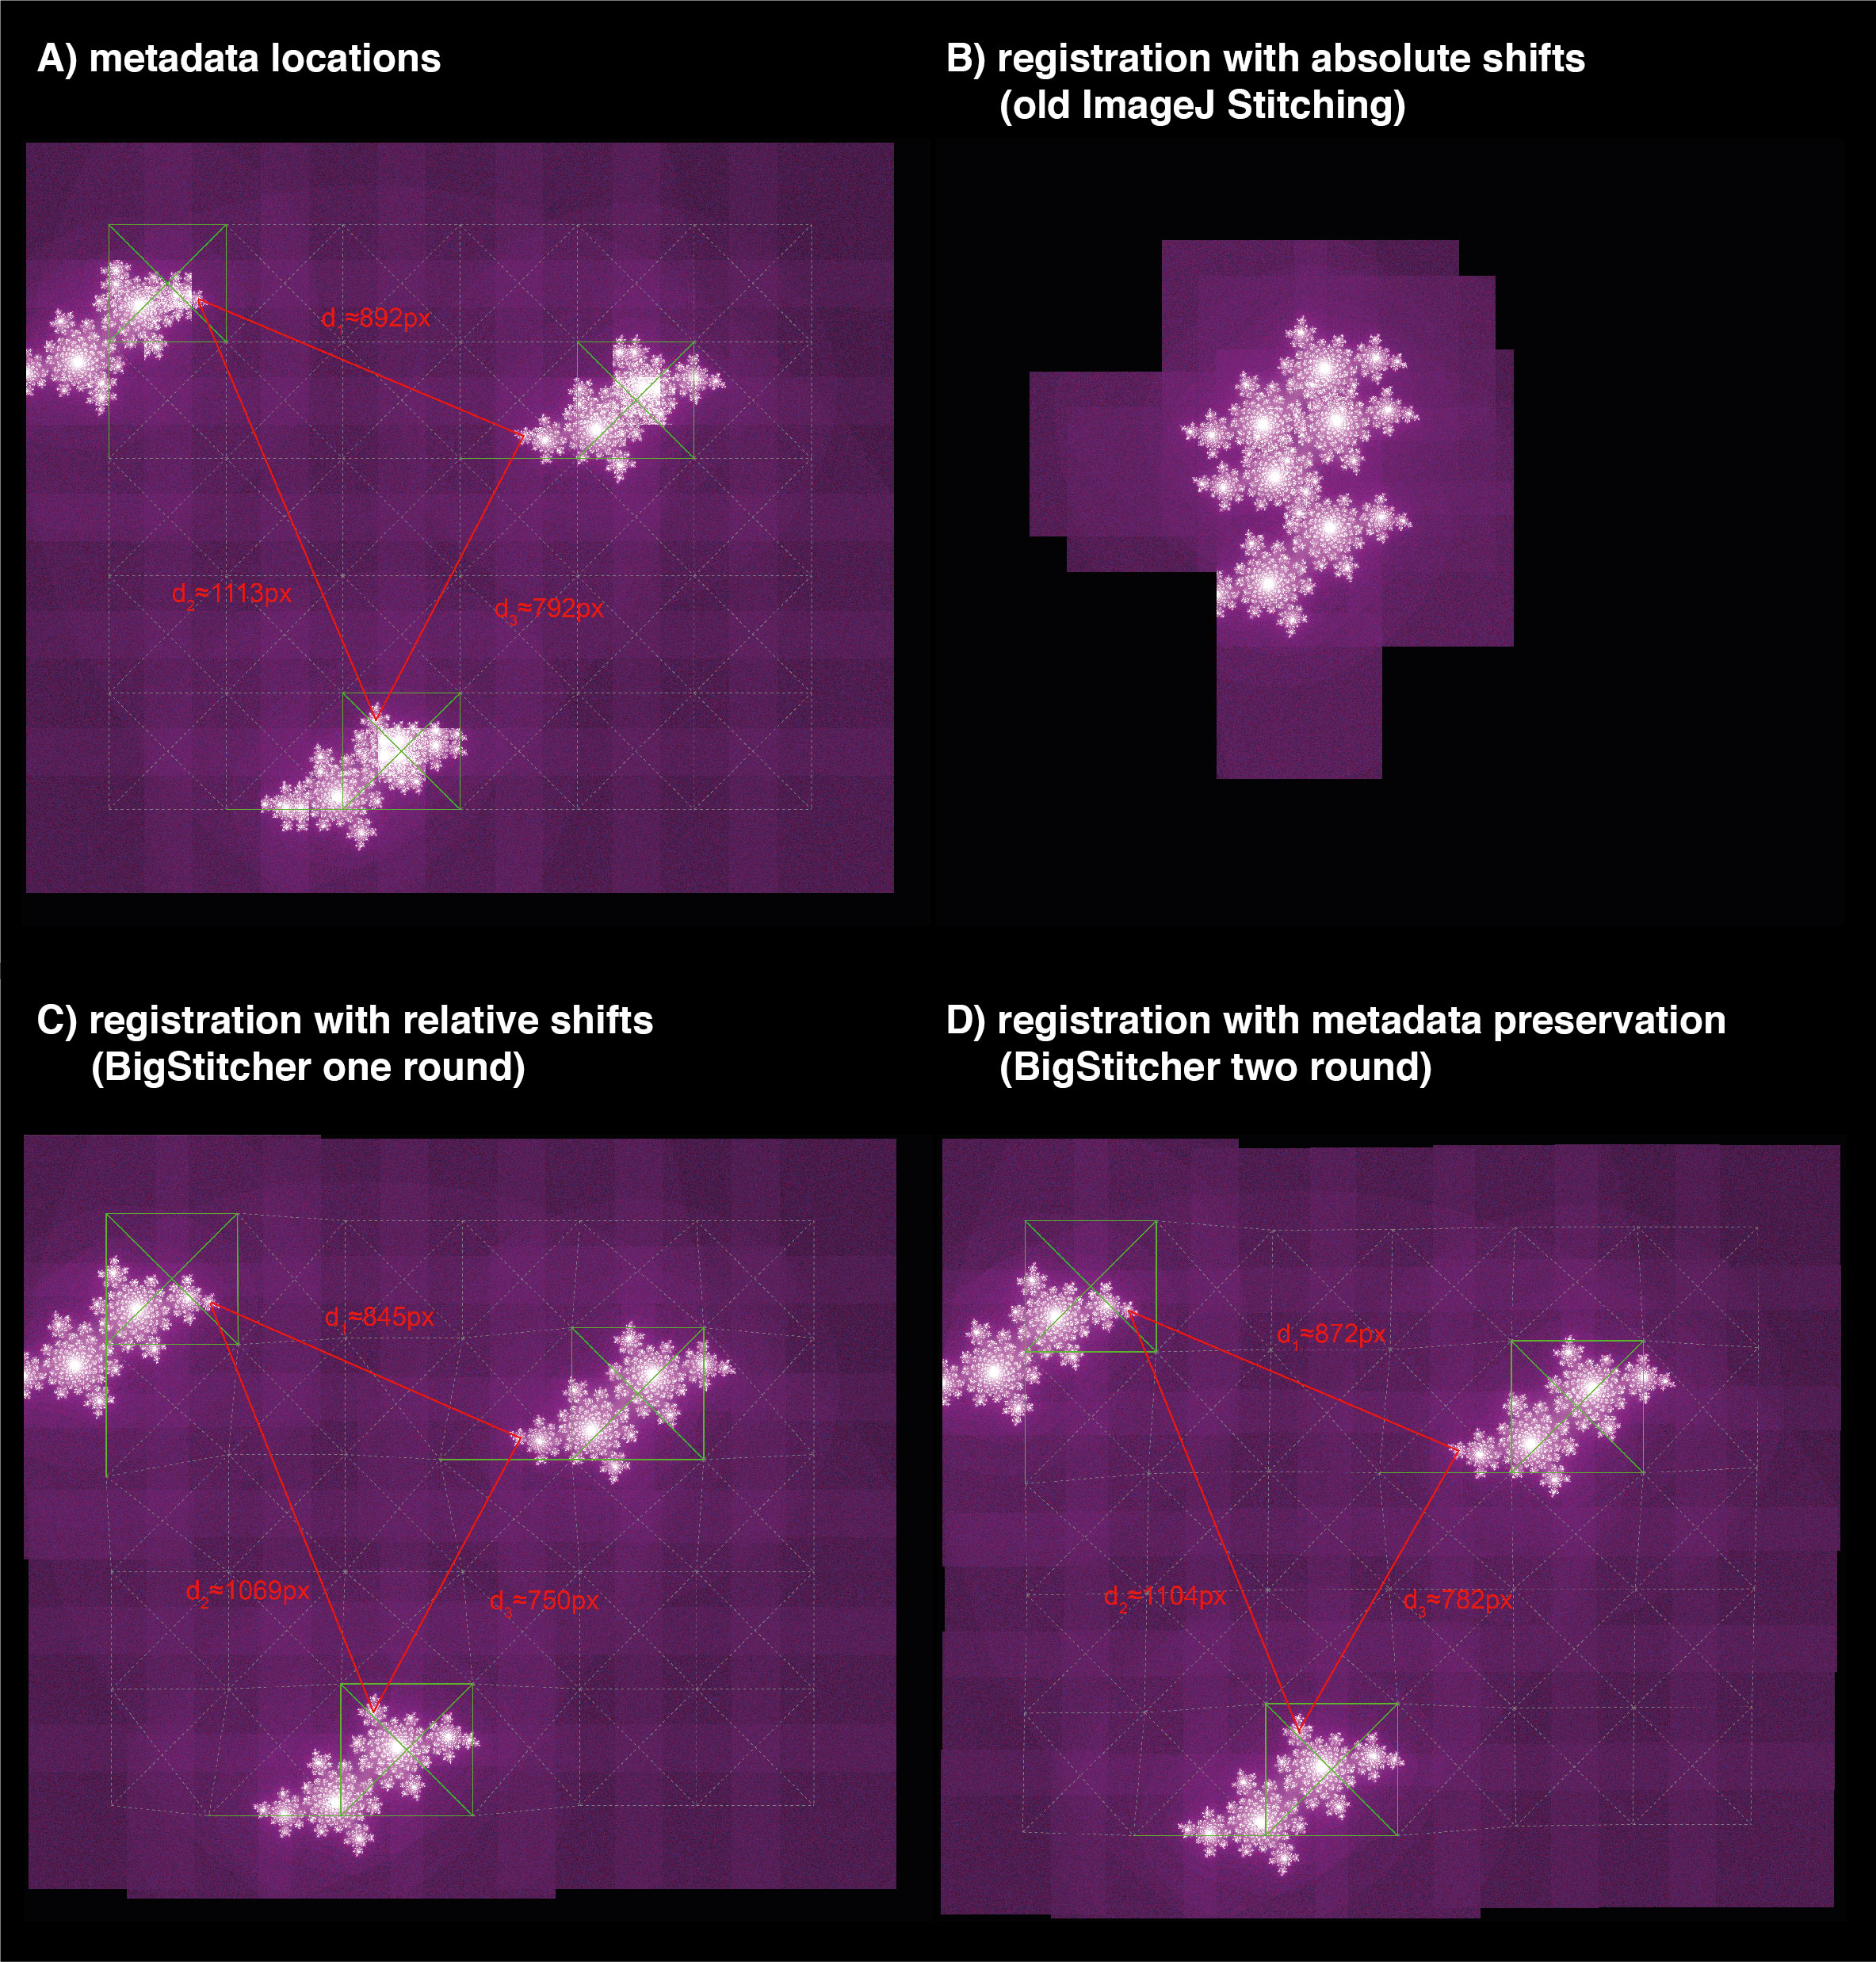
\includegraphics[width=0.85\textwidth]{fig-globalopt.png}}
\vspace{2.0mm}
\caption{\hspace{-0.5mm} \emph{Global optimization of pairwise registration in sparse datasets.} \textbf{(A):} Simulation of a tiled image dataset with sparse objects: tiled images of multiple translated Julia fractals moved to a grid according to approximate metadata (with too high overlap). Centers of images for which pairwise shifts can be determined via phase correlation are connected by green lines, whereas centers of neighboring tiles for which no meaningful shift can be calculated are linked by dashed grey lines. Manually measured distances between distinct points in the three fractals are shown in red. Performing global optimization with \emph{absolute shifts} (as it is done BigStitcher's predecessor, the ImageJ Stitching plugin) will correctly align images within connected components of the link graph but place all fractals close to the origin \textbf{(B)}. By using \emph{relative shifts}, BigStitcher will leave disconnected objects at their initial location while still aligning within connected components \textbf{(C)}. As registrations are not propagated between unconnected tiles, distances between neighboring objects might change. By running a second round of optimization to align connected components according to metadata shifts and applying the results to the in-component registrations, distances between neighboring objects are preserved as-well-as-possible \textbf{(D)}.
}
\label{fig:sup-fig-globalopt}
\end{figure*}

\pagebreak


\subsection*{SUPPLEMENTARY FIGURE 11: Affine refinement via ICP}
\vspace{1mm}
\begin{figure*}[h!]
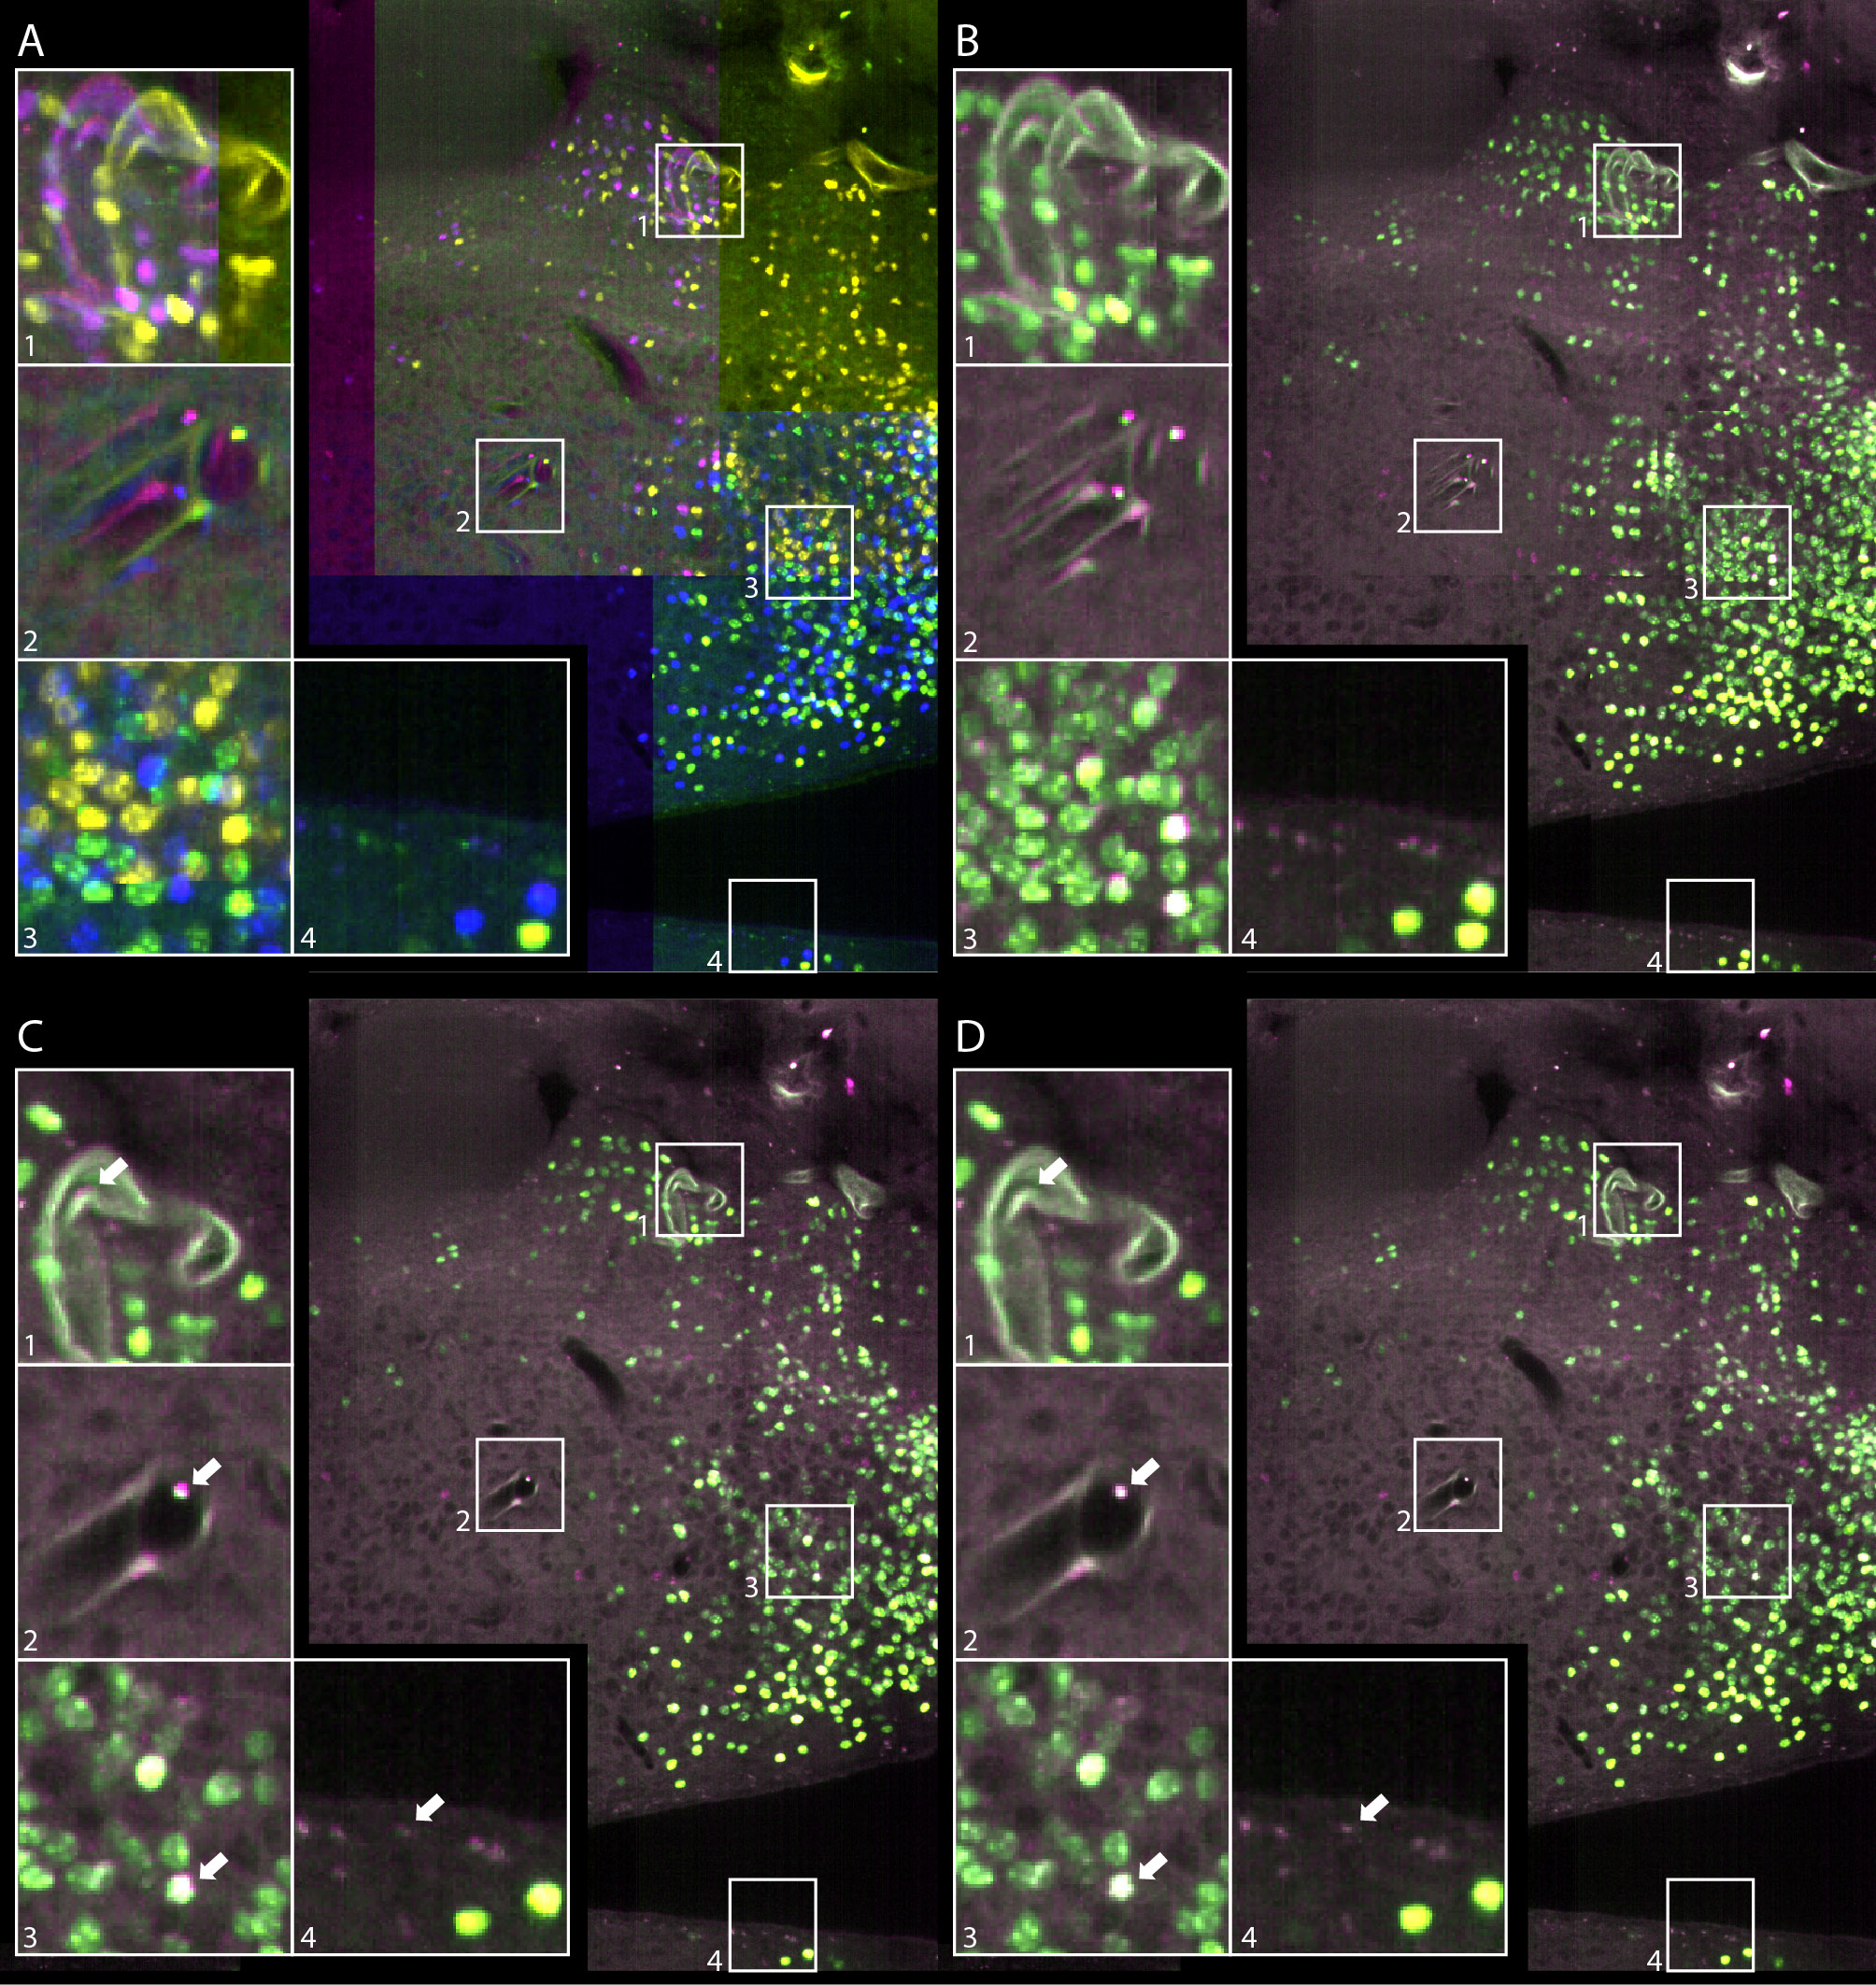
\includegraphics[width=\textwidth]{fig-stitching_icp.png}
\vspace{-2.0mm}
\caption{\hspace{-0.5mm} \emph{Lorem ipsum.} Dolor sit amet.
}
\label{fig:sup-fig-icp}
\end{figure*}

\pagebreak


\subsection*{SUPPLEMENTARY FIGURE 12: Interest Point visualization}
\vspace{1mm}
\begin{figure*}[h!]
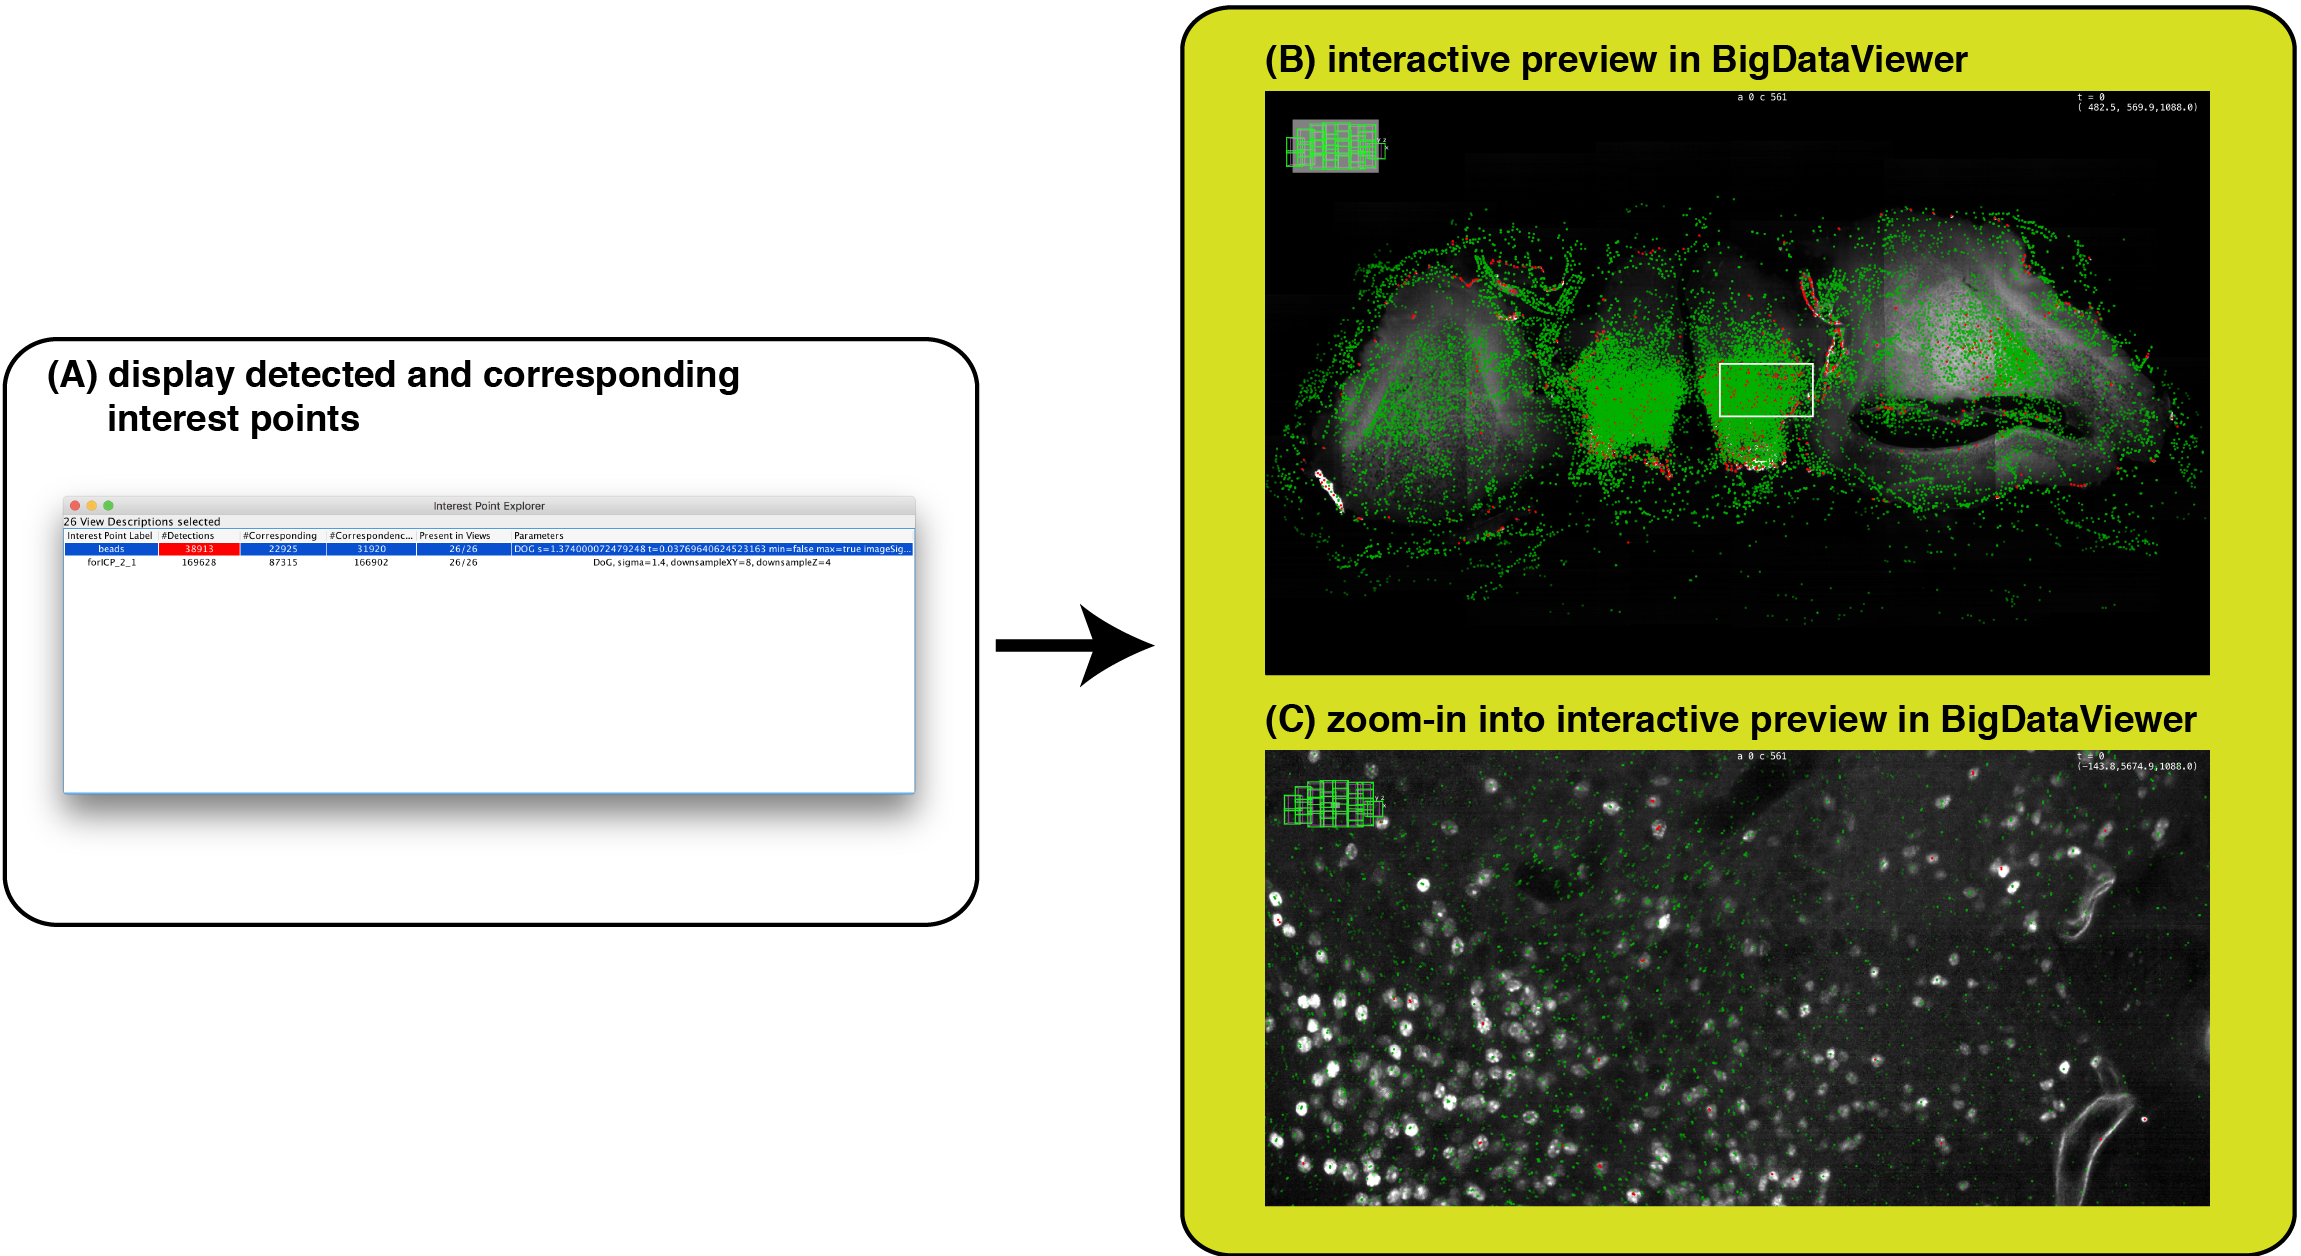
\includegraphics[width=\textwidth]{Supp-IntrestPoints.png}
\vspace{-2.0mm}
\caption{\hspace{-0.5mm} \emph{Lorem ipsum.} Dolor sit amet.
}
\label{fig:sup-fig-interest-point}
\end{figure*}

\pagebreak


\subsection*{SUPPLEMENTARY FIGURE 13: Manual Transformation of multi-view datasets}
\vspace{1mm}
\begin{figure*}[h!]
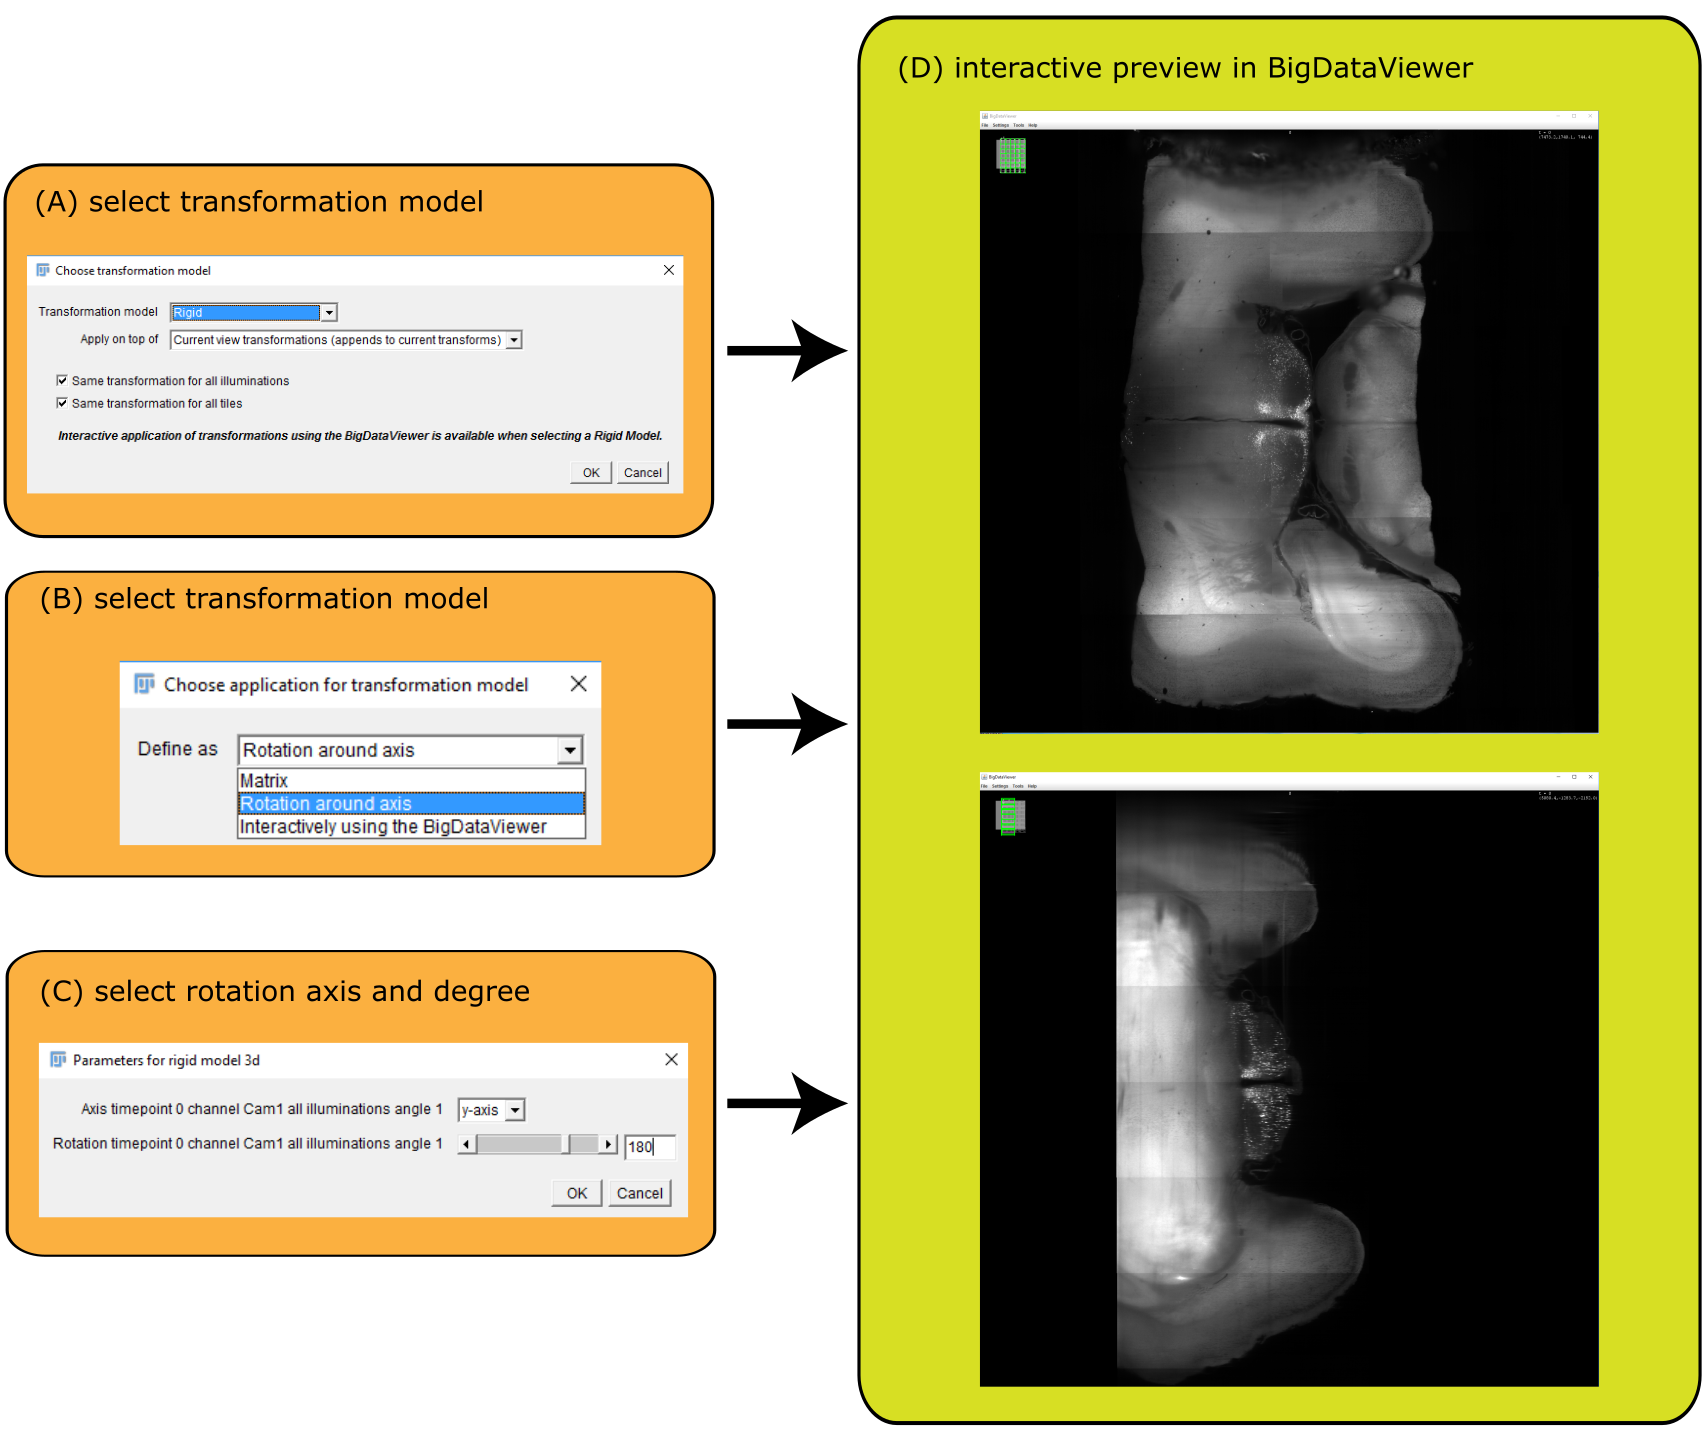
\includegraphics[width=\textwidth]{Supp-Transformation.png}
\vspace{-2.0mm}
\caption{\hspace{-0.5mm} \emph{Lorem ipsum.} Dolor sit amet.
}
\label{fig:sup-fig-manual-align2}
\end{figure*}

\pagebreak

\subsection*{SUPPLEMENTARY FIGURE 14: Bounding Box definition}
\vspace{1mm}
\begin{figure*}[h!]
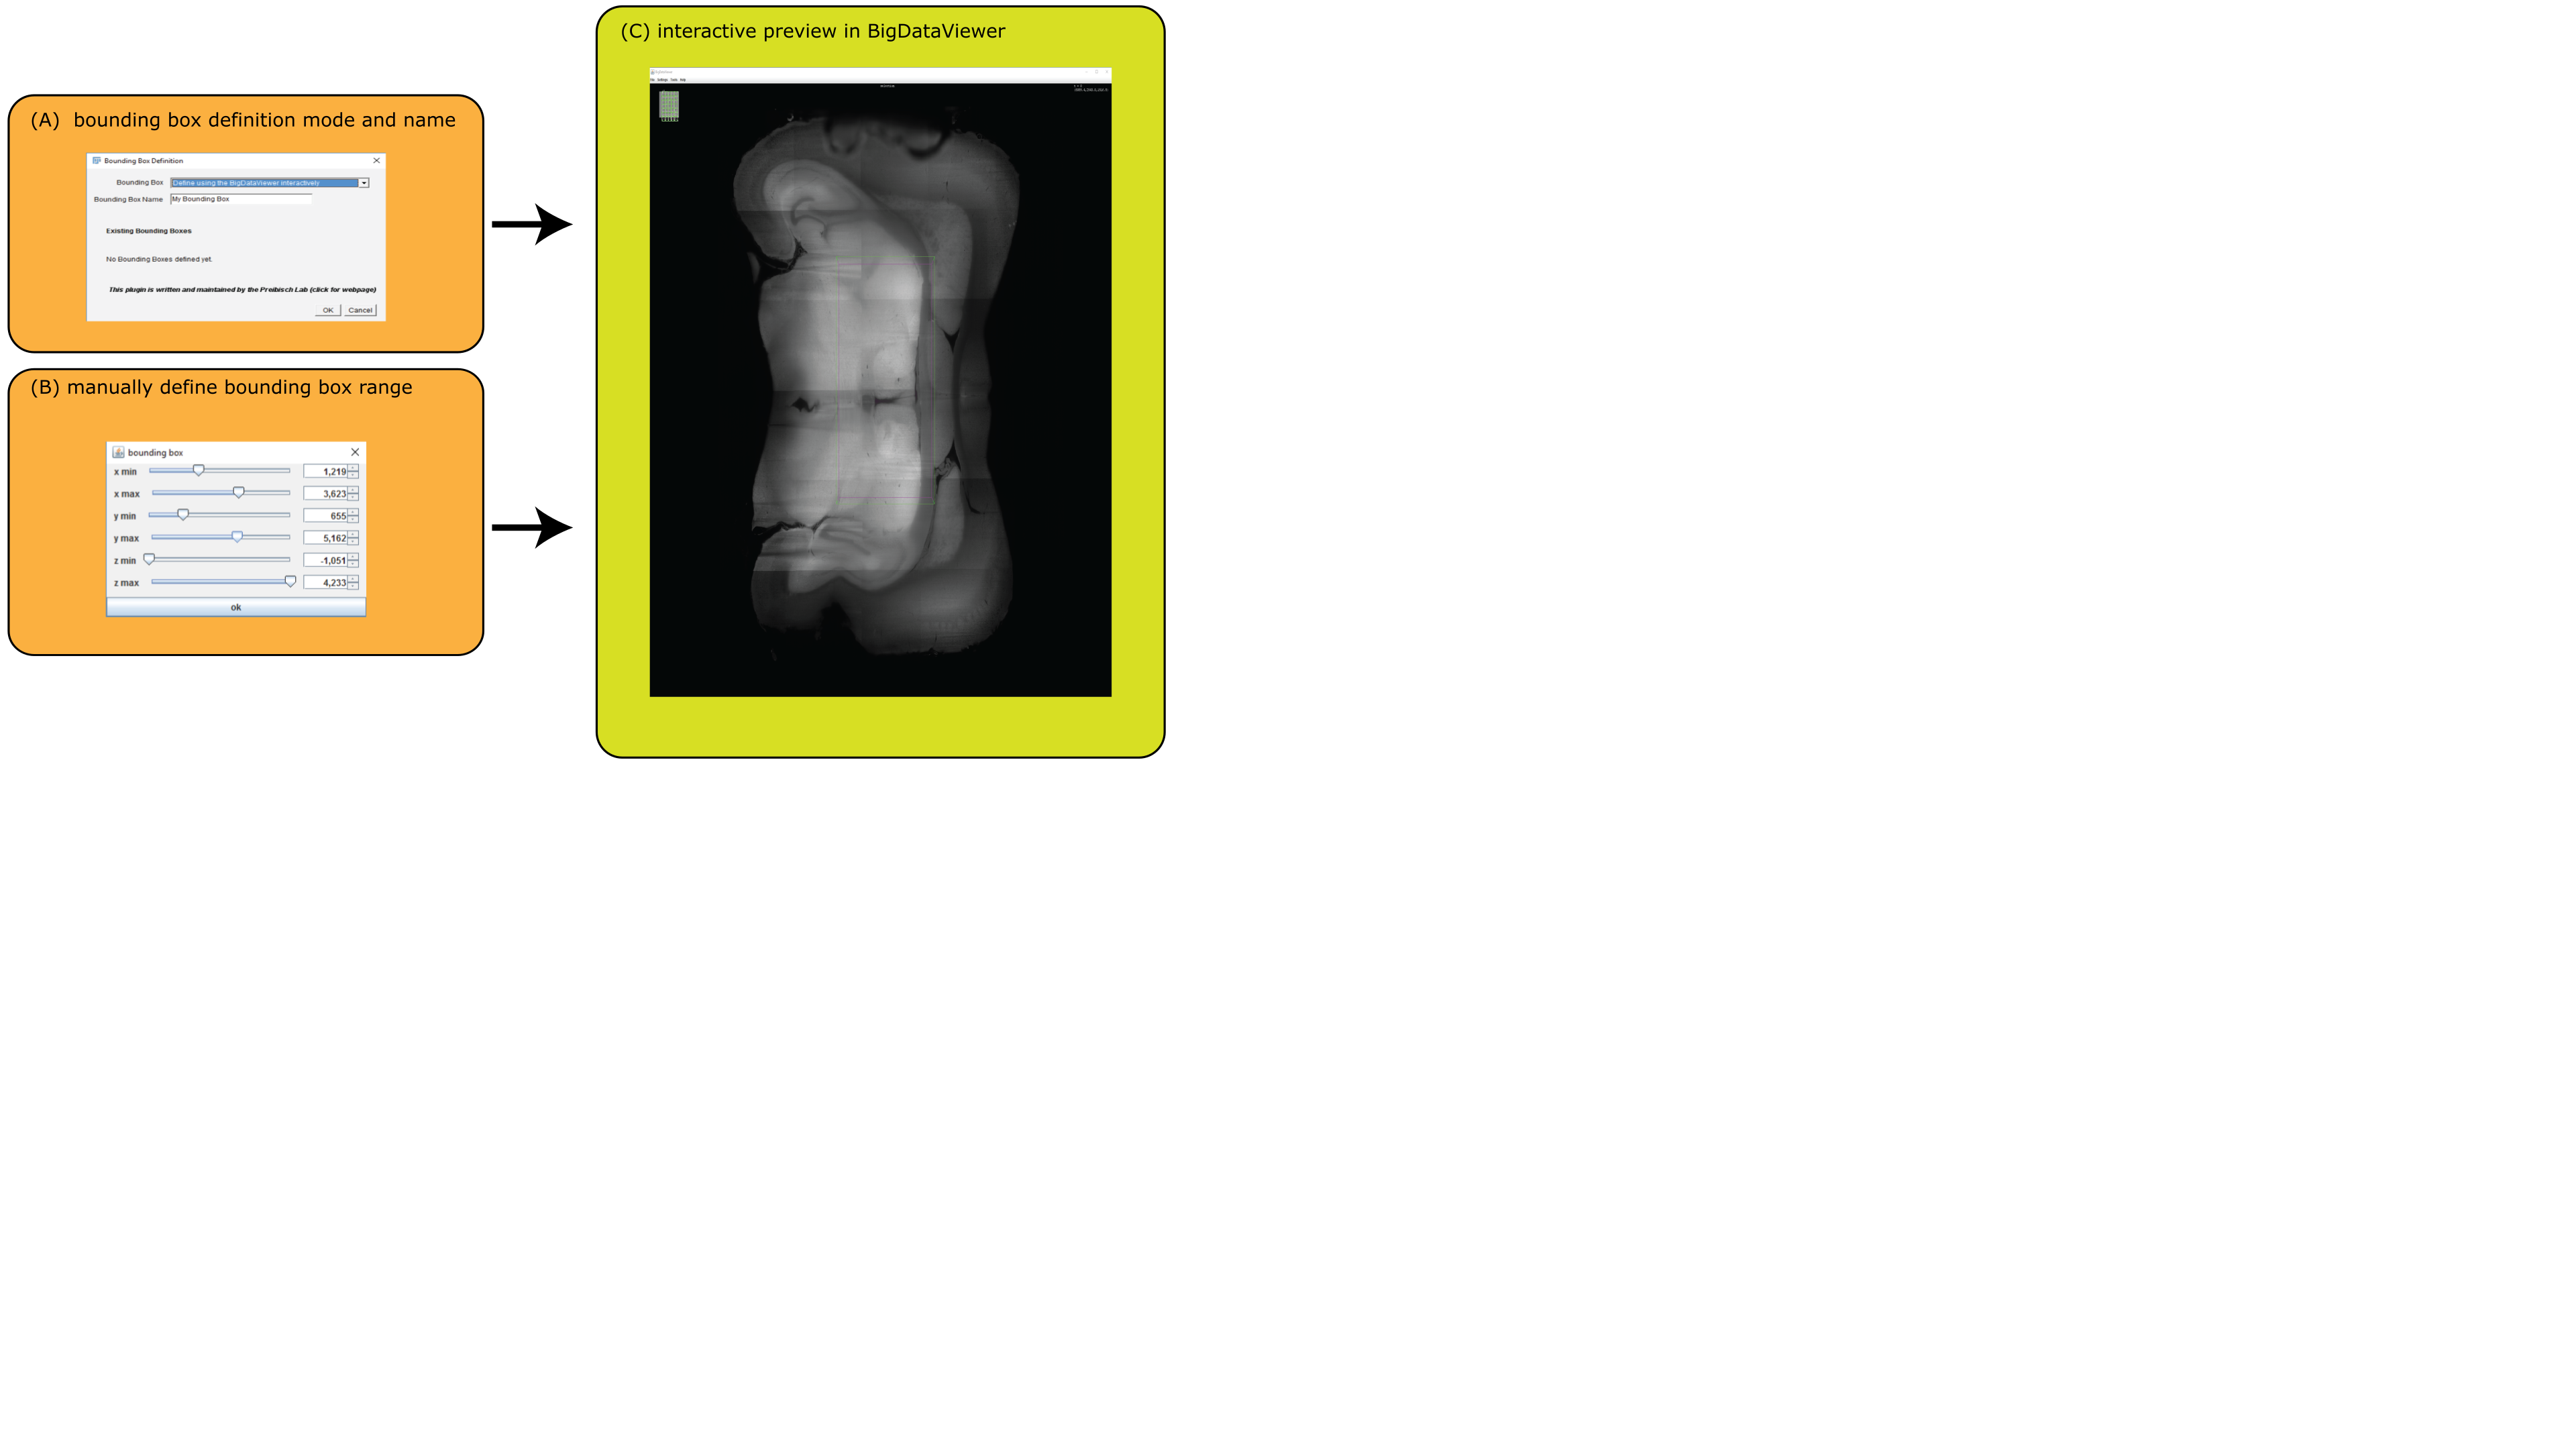
\includegraphics[width=\textwidth]{Supp-BB.png}
\vspace{-2.0mm}
\caption{\hspace{-0.5mm} \emph{Lorem ipsum.} Dolor sit amet.
}
\label{fig:sup-fig-boundingbox}
\end{figure*}

\pagebreak


\subsection*{SUPPLEMENTARY FIGURE 15: Virtual Fusion of large image}
\vspace{1mm}
\begin{figure*}[h!]
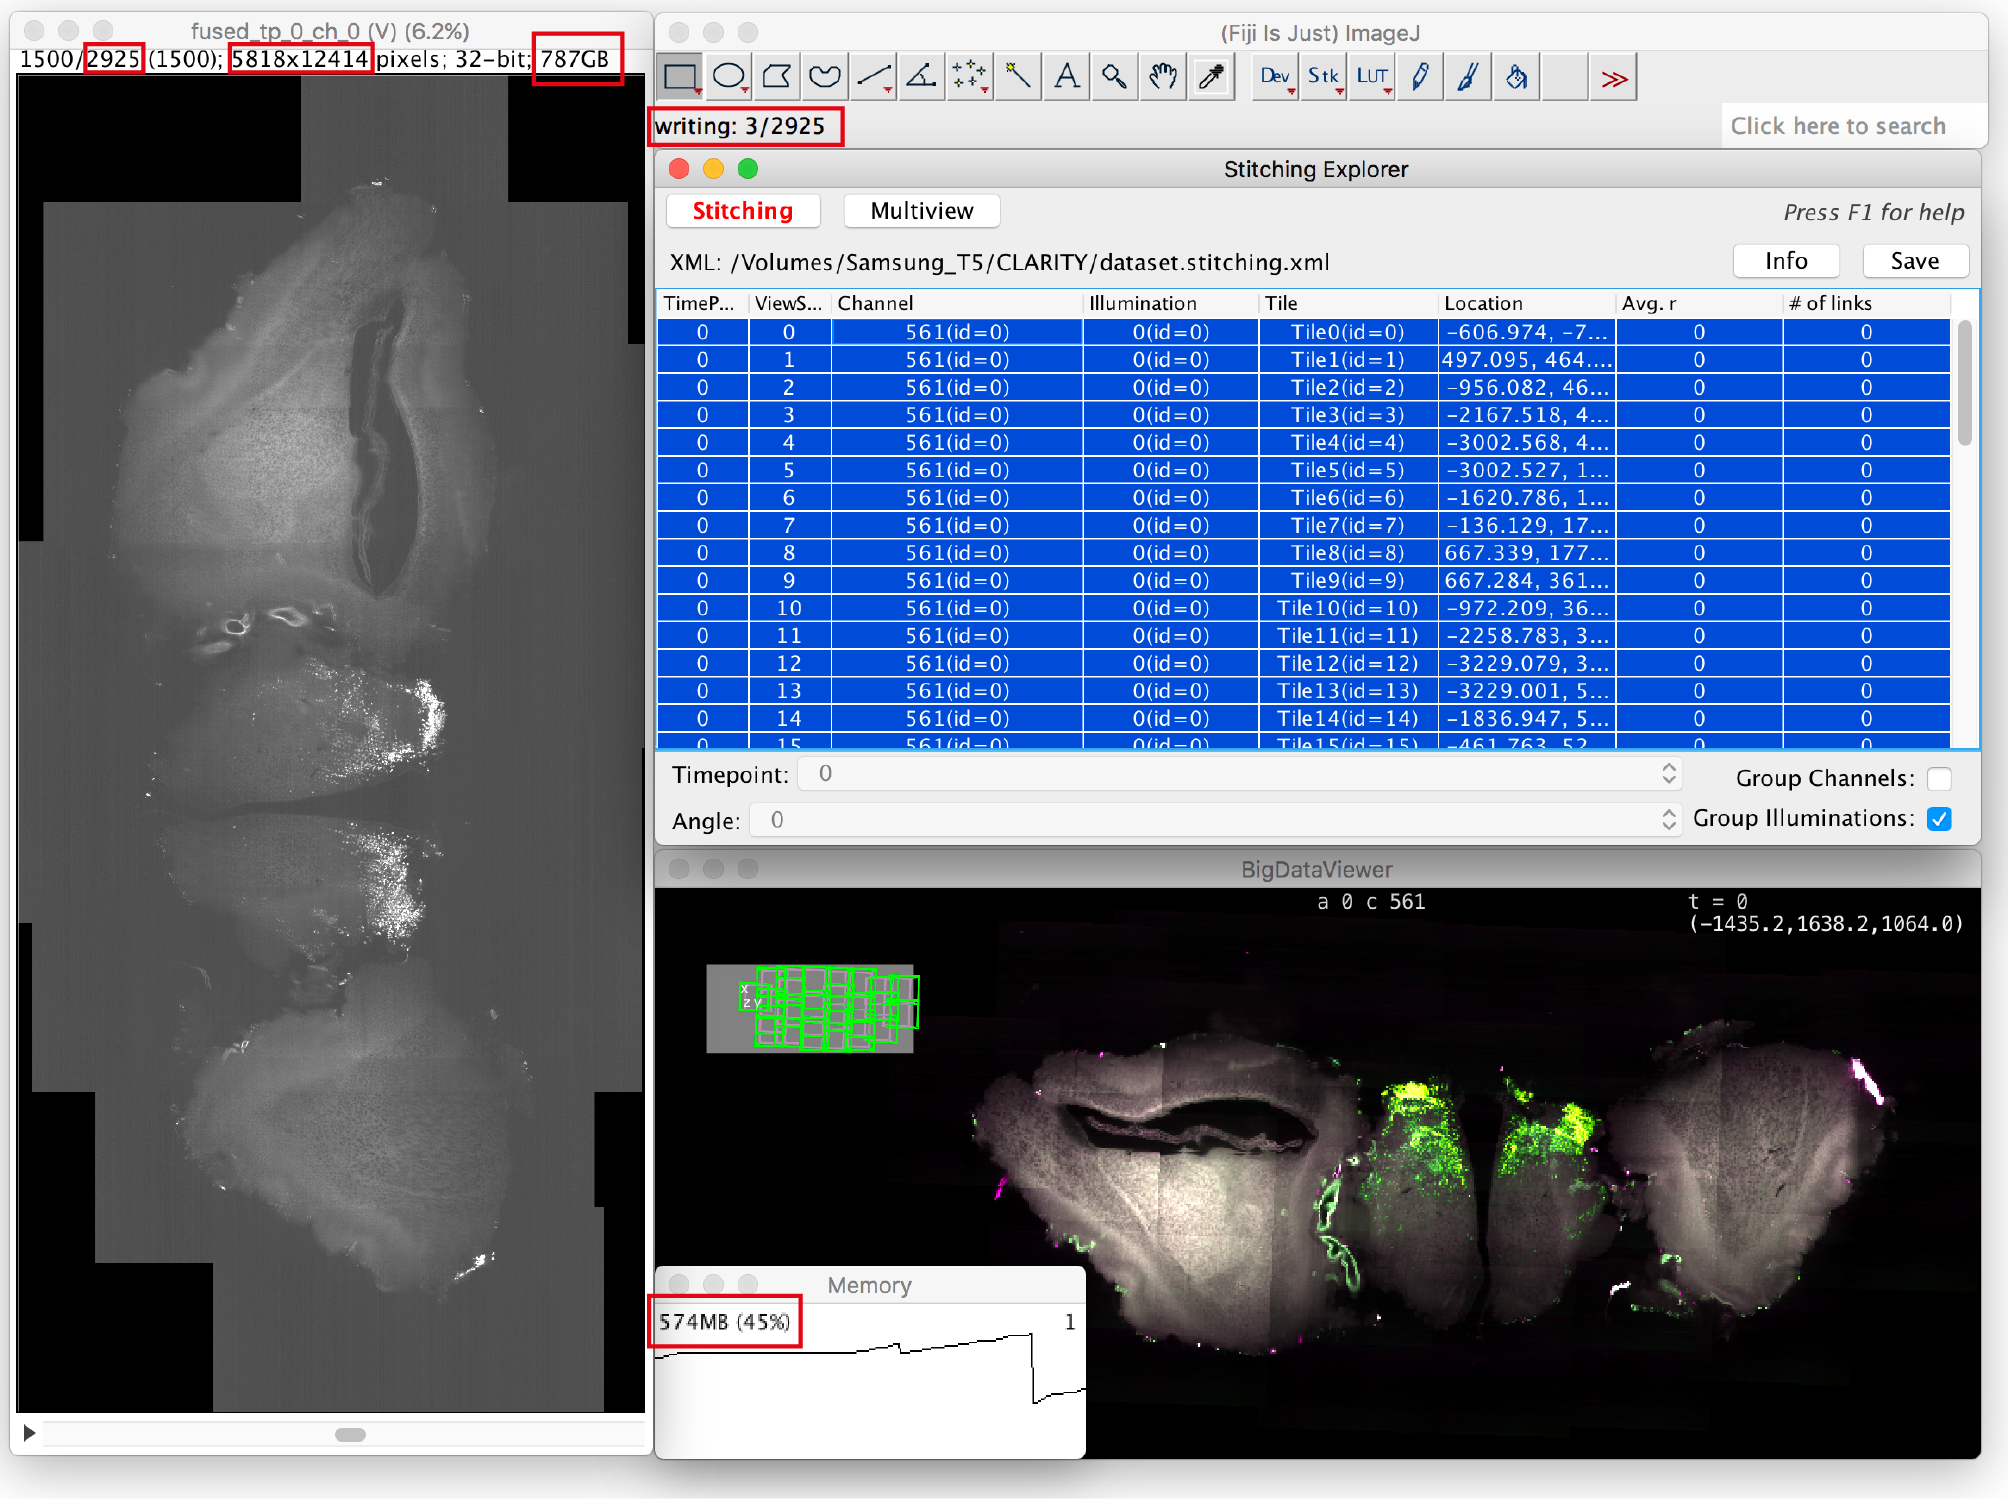
\includegraphics[width=\textwidth]{fig-fusion-screenshot.png}
\vspace{-2.0mm}
\caption{\hspace{-0.5mm} \emph{Lorem ipsum.} Dolor sit amet.
}
\label{fig:sup-fig-fusion}
\end{figure*}

\pagebreak


%========old table========
\begin{comment}

\titleformat{\section}{\centering\normalfont\fontsize{11.5pt}{1em}\bfseries}{SUPPLEMENTARY NOTE \thesection: }{0em}{}
\section*{SUPPLEMENTARY TABLES}
\titleformat{\section}{\normalfont\fontsize{11.5pt}{1em}\bfseries}{SUPPLEMENTARY NOTE \thesection: }{0em}{}



\hspace{20mm}

\subsection*{SUPPLEMENTARY TABLE 1: Summary of datasets used in this publication}

\hspace{20mm}

\setcounter{table}{0}
\newcounter{savecntr1}% Save footnote counter
\newcounter{restorecntr1}% Restore footnote counter
\newcounter{savecntr2}% Save footnote counter
\newcounter{restorecntr2}% Restore footnote counter

\begin{savenotes}
\begin{table}[h!]
\center
{
\fontsize{9pt}{10pt}\selectfont
\center
\begin{tabular}{p{5.5cm}p{3.0cm}p{3.6cm}p{3.5cm}}
\textbf{Dataset} & \textbf{Size, Lightsheet} & \textbf{Computation Time,} & \textbf{Machine}\\
 & \textbf{Thickness, SNR\footnote{The SNR is estimated by M.S., E.M., and P.T. were additionally supported by the Bundesministerium für Bildung und Forschung grant 031A099.computing the average intensity of the signal, divided by the standard deviation of the signal in areas with homogenous sample intensity}}  &\textbf{Iterations, Method} &  \\
\\
\hline
\\
\emph{Drosophila} embryo expressing His-YFP in all cells  acquired with Zeiss SPIM prototype using a 20x/0.5 detection objective (\textbf{Fig. 2c-e}, \textbf{Supp. Fig. \ref{fig:resolution}})\setcounter{savecntr1}{\value{footnote}}\footnote{This SPIM acquisition was already used in Preibisch (2010)\cite{Preibisch2010} to illustrate the results of the bead-based registration and multi-view fusion; we use the underlying dataset again to illustrate the improved results of the multi-view deconvolution.} & \mbox{720$\times$380$\times$350~px}, \mbox{7~views}, \mbox{LS$\sim$5$\mu$m, SNR$\sim$30} & \mbox{7~minutes,~~~~~~~~~~~~~~~~} \mbox{12 iterations}, \mbox{optimization I}, $\lambda$~=~0.006 & \mbox{\textcolor{red}{2$\times$~Nvidia~Quadro~4000}\setcounter{savecntr2}{\value{footnote}}\footnote{Two graphics cards in one PC, which can process two 512$\times$512$\times$512 blocks in parallel}}, 64~GB RAM\\
\\
\emph{Drosophila} embryo expressing His-YFP in all cells acquired with the OpenSPIM using a 20x/0.5 detection objective (\textbf{Supp. Fig. \ref{fig:openspim}}) & \mbox{793$\times$384$\times$370~px}, \mbox{6~views}, \mbox{LS$\sim$10$\mu$m, SNR$\sim$15} & \mbox{12 minutes\footnote{Note that the increased computation time is due to larger anisotropy of the acquired stacks leading to larger effective PSF sizes, which increases  computational effort. The image could therefore not be split up into two \mbox{512$\times$512$\times$512} blocks.},~~~~~~~~~~~~~~~~} \mbox{12 iterations}, \mbox{optimization I}, $\lambda$~=~0.006 & \mbox{\textcolor{red}{2$\times$~Nvidia~Quadro~4000}}\setcounter{restorecntr2}{\value{footnote}}\setcounter{footnote}{\value{savecntr2}}\footnotemark \setcounter{footnote}{\value{restorecntr2}}, 64~GB RAM\\
\\
\emph{Drosophila} ovaries acquired on the Zeiss SPIM prototype using a 20x/0.5 detection objective (\textbf{Supp. Fig. \ref{fig:eggchamber}}) & \mbox{1211$\times$822$\times$430~px}, \mbox{12 views}, \mbox{LS$\sim$5$\mu$m, SNR$\sim$19} & \mbox{36 minutes,~~~~~~~~~~~~~~~~} \mbox{12 iterations}, \mbox{optimization I}, $\lambda$~=~0.006  & \mbox{\textcolor{red}{2$\times$~Nvidia~Quadro~4000}}\setcounter{restorecntr2}{\value{footnote}}\setcounter{footnote}{\value{savecntr2}}\footnotemark \setcounter{footnote}{\value{restorecntr2}}, 64~GB RAM \\
\\
\emph{Drosophila} embryo expressing His-YFP in all cells acquired with Zeiss SPIM prototype using a 20x/0.5 detection objective (\textbf{Supp. Video 8-10},\textbf{Supp. Fig. \ref{fig:SIM}}) & \mbox{792$\times$320$\times$310~px}, \mbox{6~views}, \mbox{236 timepoints}, \mbox{LS$\sim$5$\mu$m, SNR$\sim$26} & \mbox{24.3 hours,~~~~~~~~~~~~~~~~} \mbox{12 iterations}, \mbox{optimization I}, $\lambda$~=~0.006 & \mbox{\textcolor{red}{2$\times$~Nvidia~Quadro~4000}}\setcounter{restorecntr2}{\value{footnote}}\setcounter{footnote}{\value{savecntr2}}\footnotemark \setcounter{footnote}{\value{restorecntr2}}, 64~GB RAM\\
\\
\emph{Drosophila} embryo expressing Histone-H2Av-mRFPruby fusion in all cells imaged on Zeiss Lightsheet Z1 with a 20x/1.0 detection objective and dual-sided illumination & \mbox{928$\times$390$\times$390~px}, \mbox{6~views}, \mbox{715~timepoints}, \mbox{LS$\sim$5$\mu$m, SNR$\sim$21} & \mbox{35 hours,~~~~~~~~~~~~~~~~} \mbox{10 iterations}, \mbox{optimization I}, $\lambda$~=~0.0006 & \mbox{\textcolor{red}{4$\times$~Nvidia~TESLA}}\footnote{Run on a cluster with 4 nodes that are equipped with one Nvidia TESLA and 64~GB of system memory}, 64~GB RAM \\
\\
\emph{C. elegans} embryo in 4-cell stage expressing PH-domain-GFP fusion acquired with Zeiss SPIM prototype using a 40x/0.8 detection objective (\textbf{Fig. 2a,b})\setcounter{restorecntr1}{\value{footnote}}\setcounter{footnote}{\value{savecntr1}}\footnotemark \setcounter{footnote}{\value{restorecntr1}} & \mbox{180$\times$135$\times$180~px}, \mbox{6~views}, \mbox{LS$\sim$3.5$\mu$m, SNR$\sim$40} & \mbox{1 minute,~~~~~~~~~~~~~~~~} \mbox{20 iterations}, \mbox{optimization I}, $\lambda$~=~0.006 & \mbox{\textcolor{blue}{2$\times$~Intel~Xeon E5-2630}}, 64~GB RAM\\
\\
Fixed \emph{C. elegans} larvae in L1 stage expressing LMN-1::GFP and stained with Hoechst imaged on Zeiss Lightsheet Z1 with a 20x/1.0 detection objective (\textbf{Fig. 2f,g} and \textbf{Supp. Video 4-7}) & \mbox{1640$\times$1070$\times$345~px}, \mbox{4 views}, \mbox{2~channels}, \mbox{LS$\sim$2$\mu$m}, \mbox{SNR$\sim$62 (Hoechst)}, \mbox{SNR$\sim$24 (GFP)} & \mbox{2$\times$160 minutes,~~~~~~~~~~~~~~~~} \mbox{100 iterations}, \mbox{optimization II}, $\lambda$~=~0 & \mbox{\textcolor{blue}{2$\times$~Intel~Xeon E5-2690}}, 128~GB RAM \\
\\
\end{tabular}}
%\nocaption
\caption{ }
\label{tab:experiments}
\end{table}
\end{savenotes}

\hspace{20mm}

\subsection*{SUPPLEMENTARY TABLE 1 (CONTINUED): Summary of datasets used in this publication}

\hspace{20mm}

\begin{savenotes}
\begin{table}[h!]
\center
{
\fontsize{9pt}{10pt}\selectfont
\center
\begin{tabular}{p{5.5cm}p{3.0cm}p{3.6cm}p{3.5cm}}
\textbf{Dataset} & \textbf{Size, Lightsheet} & \textbf{Computation Time,} & \textbf{Machine}\\
 & \textbf{Thickness, SNR}  &\textbf{Iterations, Method} &  \\
\\
\hline
\\
\emph Fixed {C. elegans} in L1 stage stained with Sytox green acquired with \textcolor{red}{Spinning Disc Confocal} using a 20x/0.5 detection objective (\textbf{Supp. Fig. \ref{fig:spinningdisc}})\footnote{This multi-view spinning disc acquisition was already used in Preibisch (2010)\cite{Preibisch2010} to illustrate the applicability of the bead-based registration and multi-view fusion to other technologies than SPIM; we use the underlying dataset again to illustrate the improved results and applicability of the multi-view deconvolution.} & \mbox{1135$\times$400$\times$430~px}, \mbox{5~views}, \mbox{LS N/A, SNR$\sim$28} & \mbox{36 minutes,~~~~~~~~~~~~~~~~} \mbox{50 iterations}, \mbox{optimization II}, $\lambda$~=~0.0006 & \mbox{\textcolor{blue}{2$\times$~Intel~Xeon E5-2680}}, 128~GB RAM\\
\\
\emph Fixed {C. elegans} in L1 stage stained with Sytox green acquired with \textcolor{red}{Spinning Disc Confocal} using a 20x/0.5 detection objective (\textbf{Supp. Fig. \ref{fig:spinningdisc}})\footnote{This is the same dataset as in the row above, but showing the time it took to compute the single-view deconvolution.} & \mbox{1151$\times$426$\times$190~px}, \textcolor{red}{\mbox{1~view}}, \mbox{LS N/A, SNR$\sim$28} & \mbox{202 minutes,~~~~~~~~~~~~~~~~} \mbox{900 iterations}, \textcolor{red}{\mbox{Lucy-Richardson}}, $\lambda$~=~0.0006 & \mbox{\textcolor{blue}{2$\times$~Intel~Xeon E5620}}, 64~GB RAM\\
\\
\emph Fixed {Drosophila} embryo stained with Sytox green acquired on the Zeiss SPIM prototype using a 20x/0.5 detection objective (\textbf{Supp. Fig. \ref{fig:twophoton}}) & \mbox{642$\times$316$\times$391~px}, \mbox{9~views}, \mbox{LS$\sim$5$\mu$m, SNR$\sim$20} & \mbox{15 minutes,~~~~~~~~~~~~~~~~} \mbox{15 iterations}, \mbox{optimization I}, $\lambda$~=~0.006 & \mbox{\textcolor{blue}{2$\times$~Intel~Xeon E5-2680}}, 128~GB RAM\\
\\
\emph Fixed {Drosophila} embryo stained with Sytox green acquired on a \textcolor{red}{Two-Photon Microscope} using a 20x/0.8 detection objective (\textbf{Supp. Fig. \ref{fig:twophoton}}) & \mbox{856$\times$418$\times$561~px}, \textcolor{red}{\mbox{1~view}}, \mbox{LS N/A, SNR$\sim$7} & \mbox{160 minutes,~~~~~~~~~~~~~~~~} \mbox{300 iterations}, \textcolor{red}{\mbox{Lucy-Richardson}}, $\lambda$~=~0.006 & \mbox{\textcolor{blue}{2$\times$~Intel~Xeon E5620}}, 64~GB RAM\\
\\
\end{tabular}}
%\nocaption
\caption{Supplementary Table 1: \emph{Summary of all datasets used in this publication}. Note that the multi-view deconvolution of the \emph{C. elegans} larvae in L1 stage (SPIM \& Spinning Disc Confocal) required an additional registration step, which is explained in the \bf{Online Methods}.}
\label{tab:experiments2}
\end{table}
\end{savenotes}

\end{comment}

\pagebreak
%========end old table========



\input supplementary-methods.tex

\section{BIGSTITCHER USER GUIDE}
\label{sec:documentation}

\subsection{This is where the documentation will go}

Lorem ipsum dolor sit amet.

\pagebreak

% description of current version location is in currentcode.tex 
\input currentcode.tex


%\section{OTHER RELATED LITERATURE}
%The field of multi-view deconvolution is large and diverse; many areas of science contribute including medical science, astronomy, microscopy and the classical computer science. Within the focus of this publications it is not possible to discuss all aspects (e.g. multi-channel deconvolution). We therefore list other publications that contributed to various aspects of multi-image deconvolution\cite{Rajagopalan1998, Giannakis2000, Flusser2003, Vieilleville2011, heintzmann2002, ShawAl89,agard1984,agard1989,verveer1998,heintzmann2000,holmes1991,blume2007}.


%%%%%%%%%%%%%%%%%%%%%%%%%%%%%%%%%%%%%%%%%%%%%%%%%%%%%%%%%%%%%
%\acknowledgments     %>>>> equivalent to \section*{ACKNOWLEDGMENTS}

%%%%%%%%%%%%%%%%%%%%%%%%%%%%%%%%%%%%%%%%%%%%%%%%%%%%%%%%%%%%%
%%%%% References %%%%%

\bibliography{supplement-bibliography}   %>>>> bibliography data in supplement-bibliography.bib
\bibliographystyle{spiebib}   %>>>> makes bibtex use spiebib.bst

\end{document}
